% Options for packages loaded elsewhere
\PassOptionsToPackage{unicode}{hyperref}
\PassOptionsToPackage{hyphens}{url}
\PassOptionsToPackage{dvipsnames,svgnames*,x11names*}{xcolor}
%
\documentclass[
  12pt,
  a4paper]{article}
\usepackage{lmodern}
\usepackage{amssymb,amsmath}
\usepackage{ifxetex,ifluatex}
\ifnum 0\ifxetex 1\fi\ifluatex 1\fi=0 % if pdftex
  \usepackage[T1]{fontenc}
  \usepackage[utf8]{inputenc}
  \usepackage{textcomp} % provide euro and other symbols
\else % if luatex or xetex
  \usepackage{unicode-math}
  \defaultfontfeatures{Scale=MatchLowercase}
  \defaultfontfeatures[\rmfamily]{Ligatures=TeX,Scale=1}
\fi
% Use upquote if available, for straight quotes in verbatim environments
\IfFileExists{upquote.sty}{\usepackage{upquote}}{}
\IfFileExists{microtype.sty}{% use microtype if available
  \usepackage[]{microtype}
  \UseMicrotypeSet[protrusion]{basicmath} % disable protrusion for tt fonts
}{}
\makeatletter
\@ifundefined{KOMAClassName}{% if non-KOMA class
  \IfFileExists{parskip.sty}{%
    \usepackage{parskip}
  }{% else
    \setlength{\parindent}{0pt}
    \setlength{\parskip}{6pt plus 2pt minus 1pt}}
}{% if KOMA class
  \KOMAoptions{parskip=half}}
\makeatother
\usepackage{xcolor}
\IfFileExists{xurl.sty}{\usepackage{xurl}}{} % add URL line breaks if available
\IfFileExists{bookmark.sty}{\usepackage{bookmark}}{\usepackage{hyperref}}
\hypersetup{
  pdftitle={ Notes on stage 1 sampling frames for a national Simple Spatial Survey Method survey in Mozambique},
  pdfauthor={Ernest Guevarra},
  colorlinks=true,
  linkcolor=blue,
  filecolor=Maroon,
  citecolor=blue,
  urlcolor=blue,
  pdfcreator={LaTeX via pandoc}}
\urlstyle{same} % disable monospaced font for URLs
\usepackage[margin=2cm]{geometry}
\usepackage{color}
\usepackage{fancyvrb}
\newcommand{\VerbBar}{|}
\newcommand{\VERB}{\Verb[commandchars=\\\{\}]}
\DefineVerbatimEnvironment{Highlighting}{Verbatim}{commandchars=\\\{\}}
% Add ',fontsize=\small' for more characters per line
\usepackage{framed}
\definecolor{shadecolor}{RGB}{248,248,248}
\newenvironment{Shaded}{\begin{snugshade}}{\end{snugshade}}
\newcommand{\AlertTok}[1]{\textcolor[rgb]{0.94,0.16,0.16}{#1}}
\newcommand{\AnnotationTok}[1]{\textcolor[rgb]{0.56,0.35,0.01}{\textbf{\textit{#1}}}}
\newcommand{\AttributeTok}[1]{\textcolor[rgb]{0.77,0.63,0.00}{#1}}
\newcommand{\BaseNTok}[1]{\textcolor[rgb]{0.00,0.00,0.81}{#1}}
\newcommand{\BuiltInTok}[1]{#1}
\newcommand{\CharTok}[1]{\textcolor[rgb]{0.31,0.60,0.02}{#1}}
\newcommand{\CommentTok}[1]{\textcolor[rgb]{0.56,0.35,0.01}{\textit{#1}}}
\newcommand{\CommentVarTok}[1]{\textcolor[rgb]{0.56,0.35,0.01}{\textbf{\textit{#1}}}}
\newcommand{\ConstantTok}[1]{\textcolor[rgb]{0.00,0.00,0.00}{#1}}
\newcommand{\ControlFlowTok}[1]{\textcolor[rgb]{0.13,0.29,0.53}{\textbf{#1}}}
\newcommand{\DataTypeTok}[1]{\textcolor[rgb]{0.13,0.29,0.53}{#1}}
\newcommand{\DecValTok}[1]{\textcolor[rgb]{0.00,0.00,0.81}{#1}}
\newcommand{\DocumentationTok}[1]{\textcolor[rgb]{0.56,0.35,0.01}{\textbf{\textit{#1}}}}
\newcommand{\ErrorTok}[1]{\textcolor[rgb]{0.64,0.00,0.00}{\textbf{#1}}}
\newcommand{\ExtensionTok}[1]{#1}
\newcommand{\FloatTok}[1]{\textcolor[rgb]{0.00,0.00,0.81}{#1}}
\newcommand{\FunctionTok}[1]{\textcolor[rgb]{0.00,0.00,0.00}{#1}}
\newcommand{\ImportTok}[1]{#1}
\newcommand{\InformationTok}[1]{\textcolor[rgb]{0.56,0.35,0.01}{\textbf{\textit{#1}}}}
\newcommand{\KeywordTok}[1]{\textcolor[rgb]{0.13,0.29,0.53}{\textbf{#1}}}
\newcommand{\NormalTok}[1]{#1}
\newcommand{\OperatorTok}[1]{\textcolor[rgb]{0.81,0.36,0.00}{\textbf{#1}}}
\newcommand{\OtherTok}[1]{\textcolor[rgb]{0.56,0.35,0.01}{#1}}
\newcommand{\PreprocessorTok}[1]{\textcolor[rgb]{0.56,0.35,0.01}{\textit{#1}}}
\newcommand{\RegionMarkerTok}[1]{#1}
\newcommand{\SpecialCharTok}[1]{\textcolor[rgb]{0.00,0.00,0.00}{#1}}
\newcommand{\SpecialStringTok}[1]{\textcolor[rgb]{0.31,0.60,0.02}{#1}}
\newcommand{\StringTok}[1]{\textcolor[rgb]{0.31,0.60,0.02}{#1}}
\newcommand{\VariableTok}[1]{\textcolor[rgb]{0.00,0.00,0.00}{#1}}
\newcommand{\VerbatimStringTok}[1]{\textcolor[rgb]{0.31,0.60,0.02}{#1}}
\newcommand{\WarningTok}[1]{\textcolor[rgb]{0.56,0.35,0.01}{\textbf{\textit{#1}}}}
\usepackage{longtable,booktabs}
% Correct order of tables after \paragraph or \subparagraph
\usepackage{etoolbox}
\makeatletter
\patchcmd\longtable{\par}{\if@noskipsec\mbox{}\fi\par}{}{}
\makeatother
% Allow footnotes in longtable head/foot
\IfFileExists{footnotehyper.sty}{\usepackage{footnotehyper}}{\usepackage{footnote}}
\makesavenoteenv{longtable}
\usepackage{graphicx,grffile}
\makeatletter
\def\maxwidth{\ifdim\Gin@nat@width>\linewidth\linewidth\else\Gin@nat@width\fi}
\def\maxheight{\ifdim\Gin@nat@height>\textheight\textheight\else\Gin@nat@height\fi}
\makeatother
% Scale images if necessary, so that they will not overflow the page
% margins by default, and it is still possible to overwrite the defaults
% using explicit options in \includegraphics[width, height, ...]{}
\setkeys{Gin}{width=\maxwidth,height=\maxheight,keepaspectratio}
% Set default figure placement to htbp
\makeatletter
\def\fps@figure{htbp}
\makeatother
\setlength{\emergencystretch}{3em} % prevent overfull lines
\providecommand{\tightlist}{%
  \setlength{\itemsep}{0pt}\setlength{\parskip}{0pt}}
\setcounter{secnumdepth}{5}
\usepackage{booktabs}
\usepackage{longtable}
\usepackage{array}
\usepackage{multirow}
\usepackage{wrapfig}
\usepackage{float}
\usepackage{colortbl}
\usepackage{pdflscape}
\usepackage{tabu}
\usepackage{threeparttable}
\usepackage{threeparttablex}
\usepackage[normalem]{ulem}
\usepackage{makecell}
\usepackage{setspace}
%\usepackage{ebgaramond}

\onehalfspacing

\graphicspath{ {figures/} }
\usepackage{booktabs}
\usepackage{longtable}
\usepackage{array}
\usepackage{multirow}
\usepackage{wrapfig}
\usepackage{float}
\usepackage{colortbl}
\usepackage{pdflscape}
\usepackage{tabu}
\usepackage{threeparttable}
\usepackage{threeparttablex}
\usepackage[normalem]{ulem}
\usepackage{makecell}
\usepackage{xcolor}
\usepackage[]{natbib}
\bibliographystyle{plainnat}

\title{\vspace{8cm} Notes on stage 1 sampling frames for a national Simple Spatial Survey Method survey in Mozambique}
\author{Ernest Guevarra}
\date{26 August 2020}

\begin{document}
\maketitle

\newpage

\newpage

\hypertarget{introduction}{%
\section{Introduction}\label{introduction}}

This document explores possible stage 1 sampling frames for a national survey in Mozambique using the Simple Spatial Sampling Method.

\hypertarget{stage-1-sampling-grid}{%
\section{Stage 1 sampling grid}\label{stage-1-sampling-grid}}

Given a boundary map of Mozambique that includes borders at the \emph{provincias} level (administrative level 1) and point locations of villages throughout the country, various stage 1 sampling grids using \texttt{d} values from 10 to 15 kms were tested.

\hypertarget{estimating-sampling-points-based-on-area-size}{%
\subsection{Estimating sampling points based on area size}\label{estimating-sampling-points-based-on-area-size}}

The number of sampling points needed for the stage 1 sampling frame can be estimated using the total area size of the survey area and dividing this by the area size of the hexagonal grid based on a specified value of \texttt{d}.

Given a specific \texttt{d} value, the area size of the hexagonal grid can be calculated as follows:

\[ \text{hexagon area size} ~ = ~ \frac{3 \times \sqrt{3}}{2} ~ d ^ 2  \]

Mozambique has a total area size of \(801590 ~ \text{km} ^ 2\). The estimated number of sampling points for a national survey in Mozambique using simple spatial sampling method is estimated by:

\[ n_\text{estimated total sampling points} ~ = ~ \frac{\text{Total area size of Mozambique}}{\text{Hexagon area size}} ~ = ~ \frac{801590 ~ \text{km} ^ 2}{\frac{3 \times \sqrt{3}}{2} ~ d ^ 2} \]

The hexagon area sizes for \texttt{d} values from 10 to 15 kms are and the corresponding number of sampling points required are shown in the table below:

\begin{table}[H]

\caption{\label{tab:calc}Hexagonal grid area sizes for d values from 10 to 15 kms}
\centering
\begin{tabular}[t]{rrr}
\toprule
d & \makecell[c]{Hexagon\\area\\size} & \makecell[c]{Number\\of\\sampling\\points}\\
\midrule
\rowcolor{gray!6}  10 & 259.81 & 3086\\
11 & 314.37 & 2550\\
\rowcolor{gray!6}  12 & 374.12 & 2143\\
13 & 439.07 & 1826\\
\rowcolor{gray!6}  14 & 509.22 & 1575\\
\addlinespace
15 & 584.57 & 1372\\
\bottomrule
\end{tabular}
\end{table}

The preceding calculations assume that the villages within Mozambique are spread througout the whole land area of the country. However, as shown in the map below, there are areas within the country with no settlements

\begin{figure}[H]

{\centering 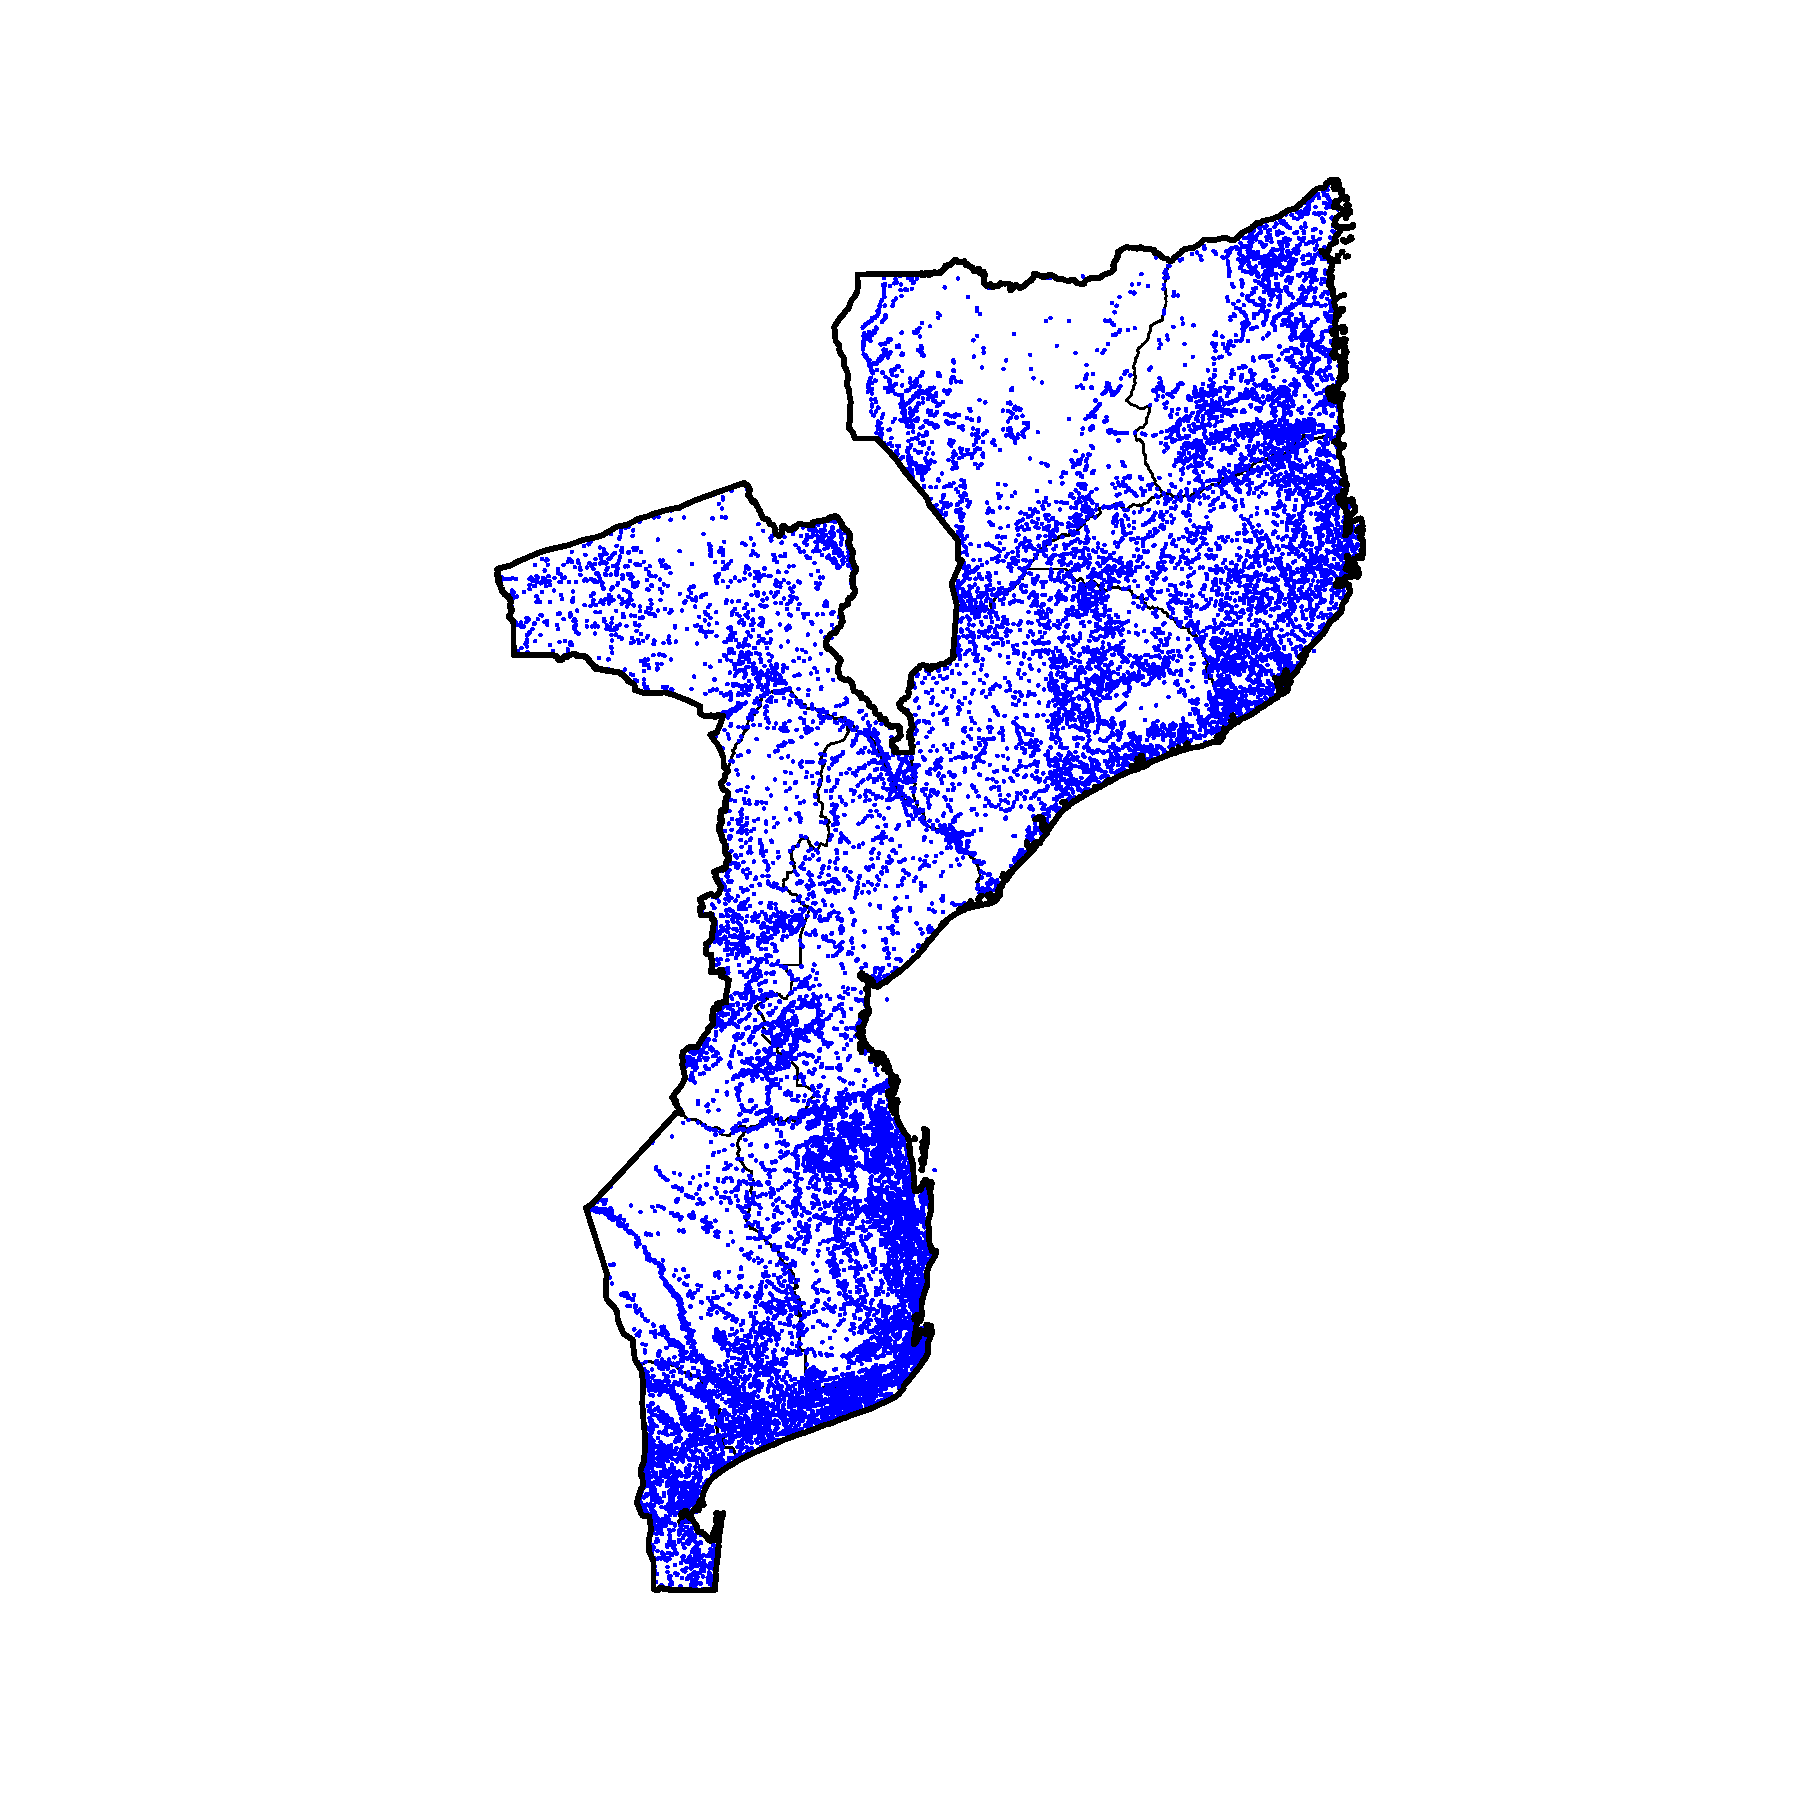
\includegraphics{mozambiqueNotes_files/figure-latex/settlementsPlot-1} 

}

\caption{Map of Mozambique provinces with settlements}\label{fig:settlementsPlot}
\end{figure}

The implication is that this estimation approach tends to overestimate the total number of sampling points needed. From a planning perspective, this can be acceptable particularly if appropriate maps for use in stage 1 sampling are still being secured. This approach provides a safe estimate to use for planning as resources will be organised based on a higher number of sampling points for the stage 1 sampling frame and eventually can be adjusted down (if needed) once a map-based determination has been performed (as described below).

\hypertarget{determining-number-of-sampling-points-using-maps}{%
\subsection{Determining number of sampling points using maps}\label{determining-number-of-sampling-points-using-maps}}

Once maps are available, number of sampling points can be determined based on the simple spatial sampling method approach to stage 1 sampling.

The various stage 1 sampling frames for values of \texttt{d} from 10 to 15 kms including respective stage 1 sampling maps are shown below.

\begin{table}[H]

\caption{\label{tab:stage1table}Stage 1 sample characteristics of various d values}
\centering
\begin{tabular}[t]{rrr}
\toprule
d & \makecell[c]{Number\\of\\sampling\\points} & \makecell[c]{Number\\of\\clusters/\\settlements\\selected}\\
\midrule
\rowcolor{gray!6}  10 & 3086 & 2727\\
11 & 2550 & 2323\\
\rowcolor{gray!6}  12 & 2143 & 2006\\
13 & 1826 & 1723\\
\rowcolor{gray!6}  14 & 1575 & 1509\\
\addlinespace
15 & 1372 & 1328\\
\bottomrule
\end{tabular}
\end{table}

As was expected, the number of sampling points based on actual maps are less than the estimated sampling points. The following maps show the selected settlements for sampling at various values for \texttt{d}.

\begin{figure}[H]

{\centering 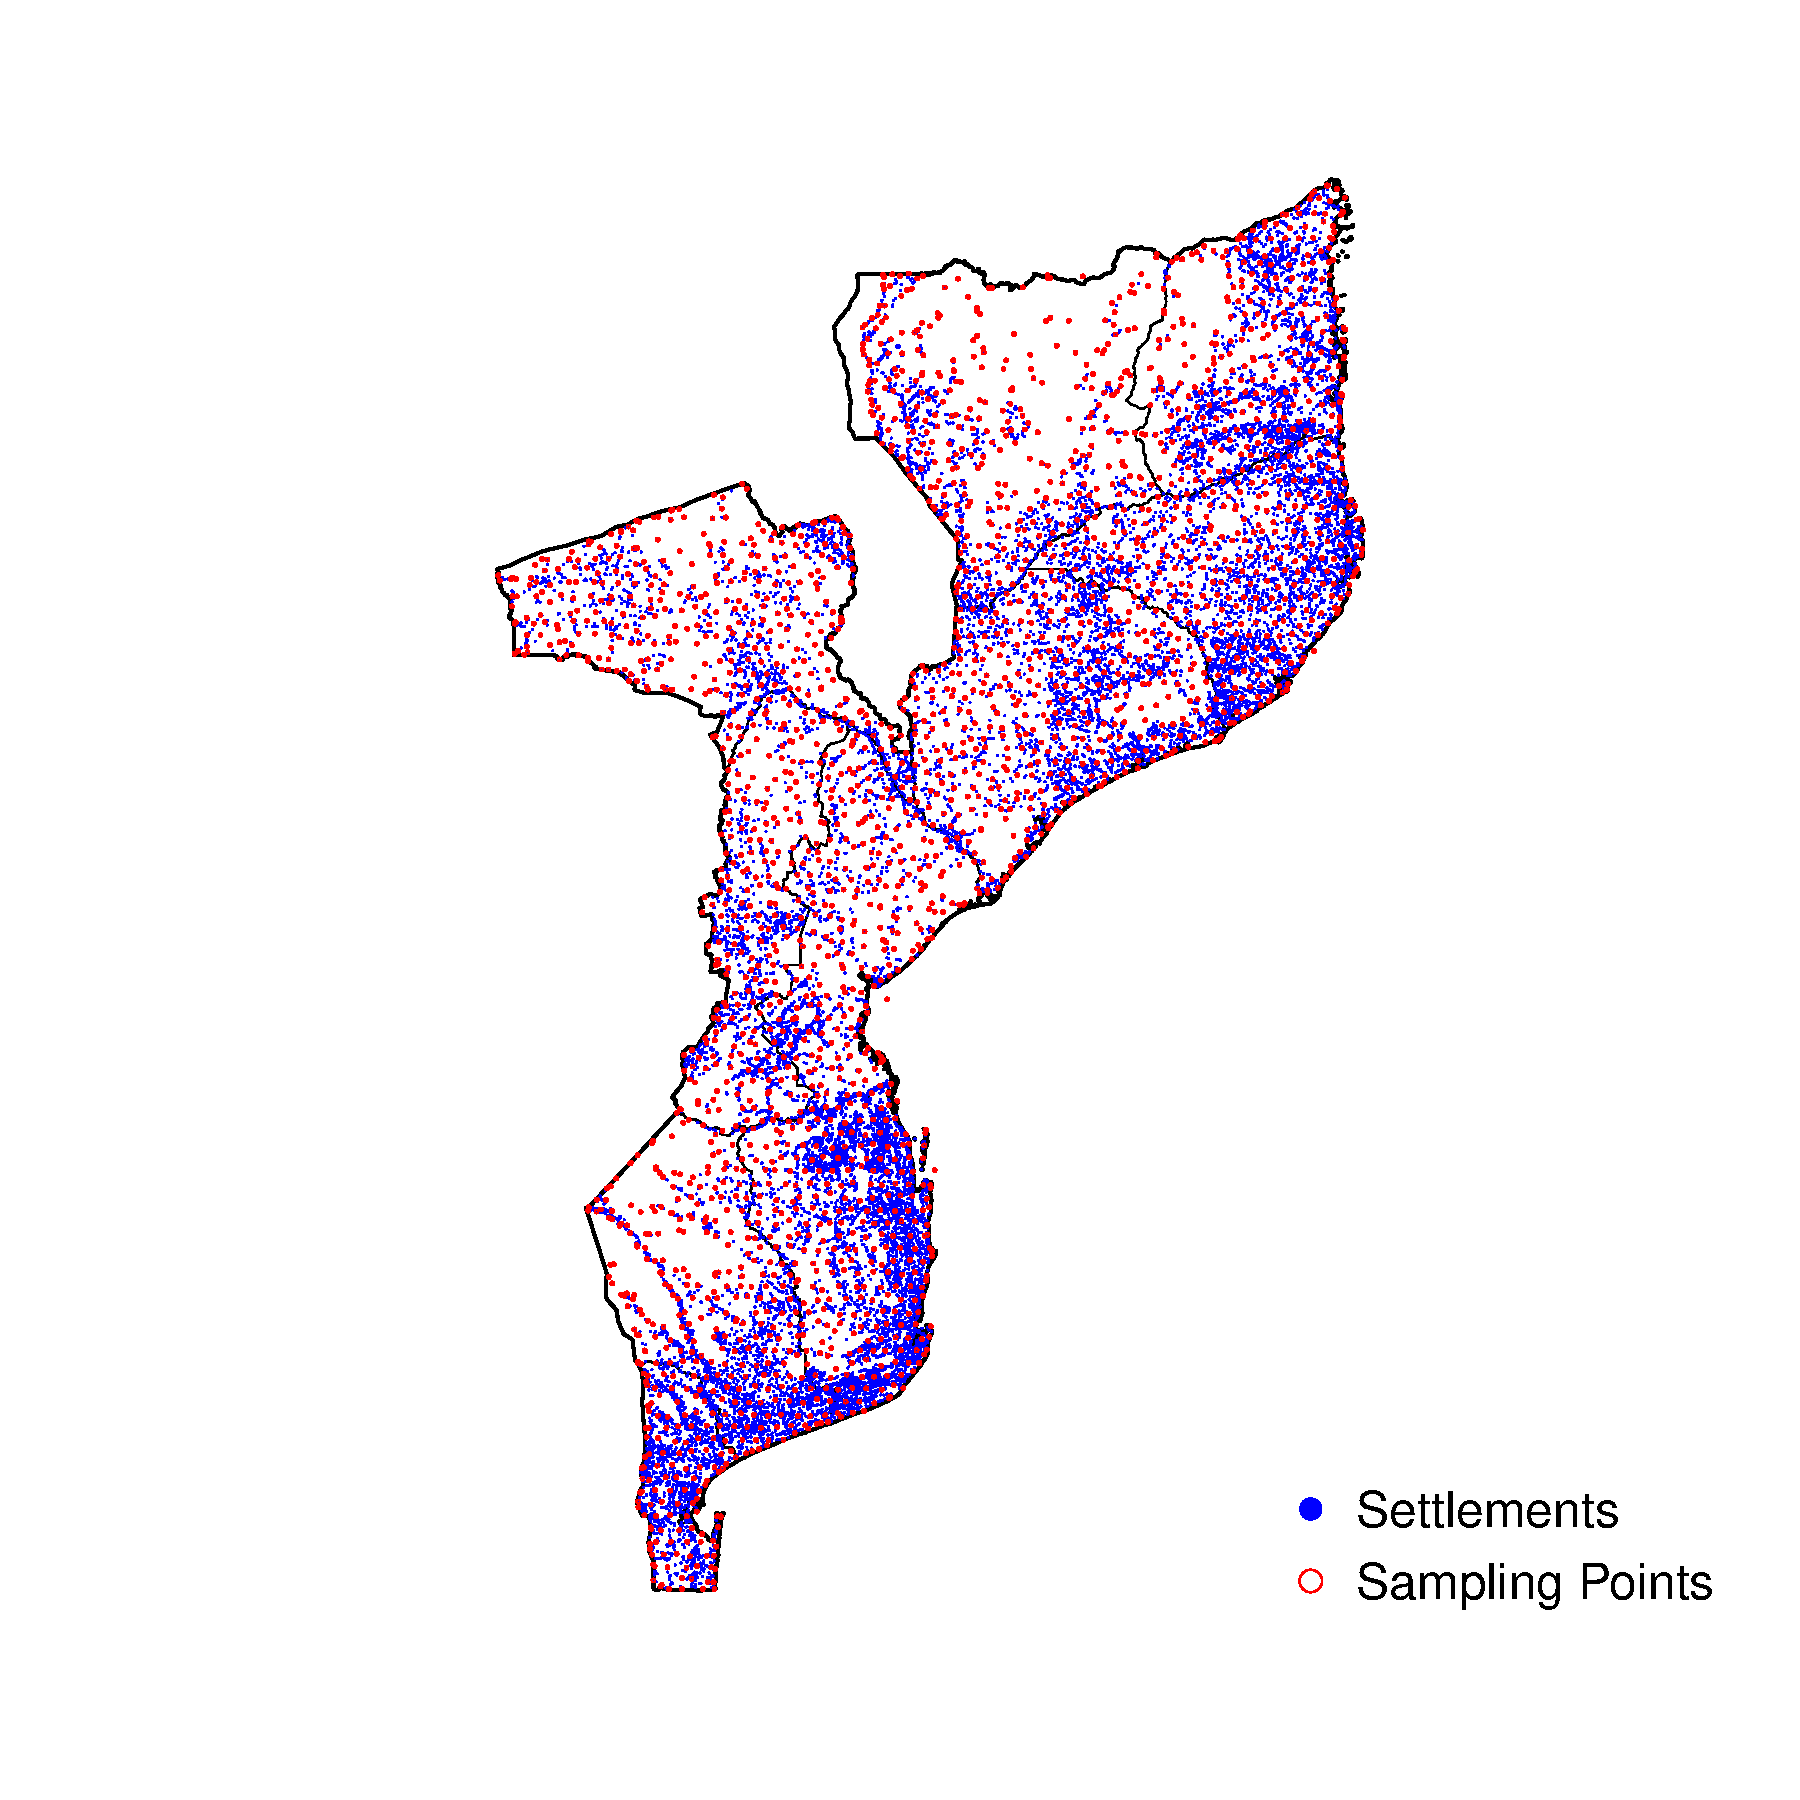
\includegraphics{mozambiqueNotes_files/figure-latex/stage1plot10-1} 

}

\caption{Stage 1 sampling map for d of 10 kms}\label{fig:stage1plot10}
\end{figure}

\begin{figure}[H]

{\centering 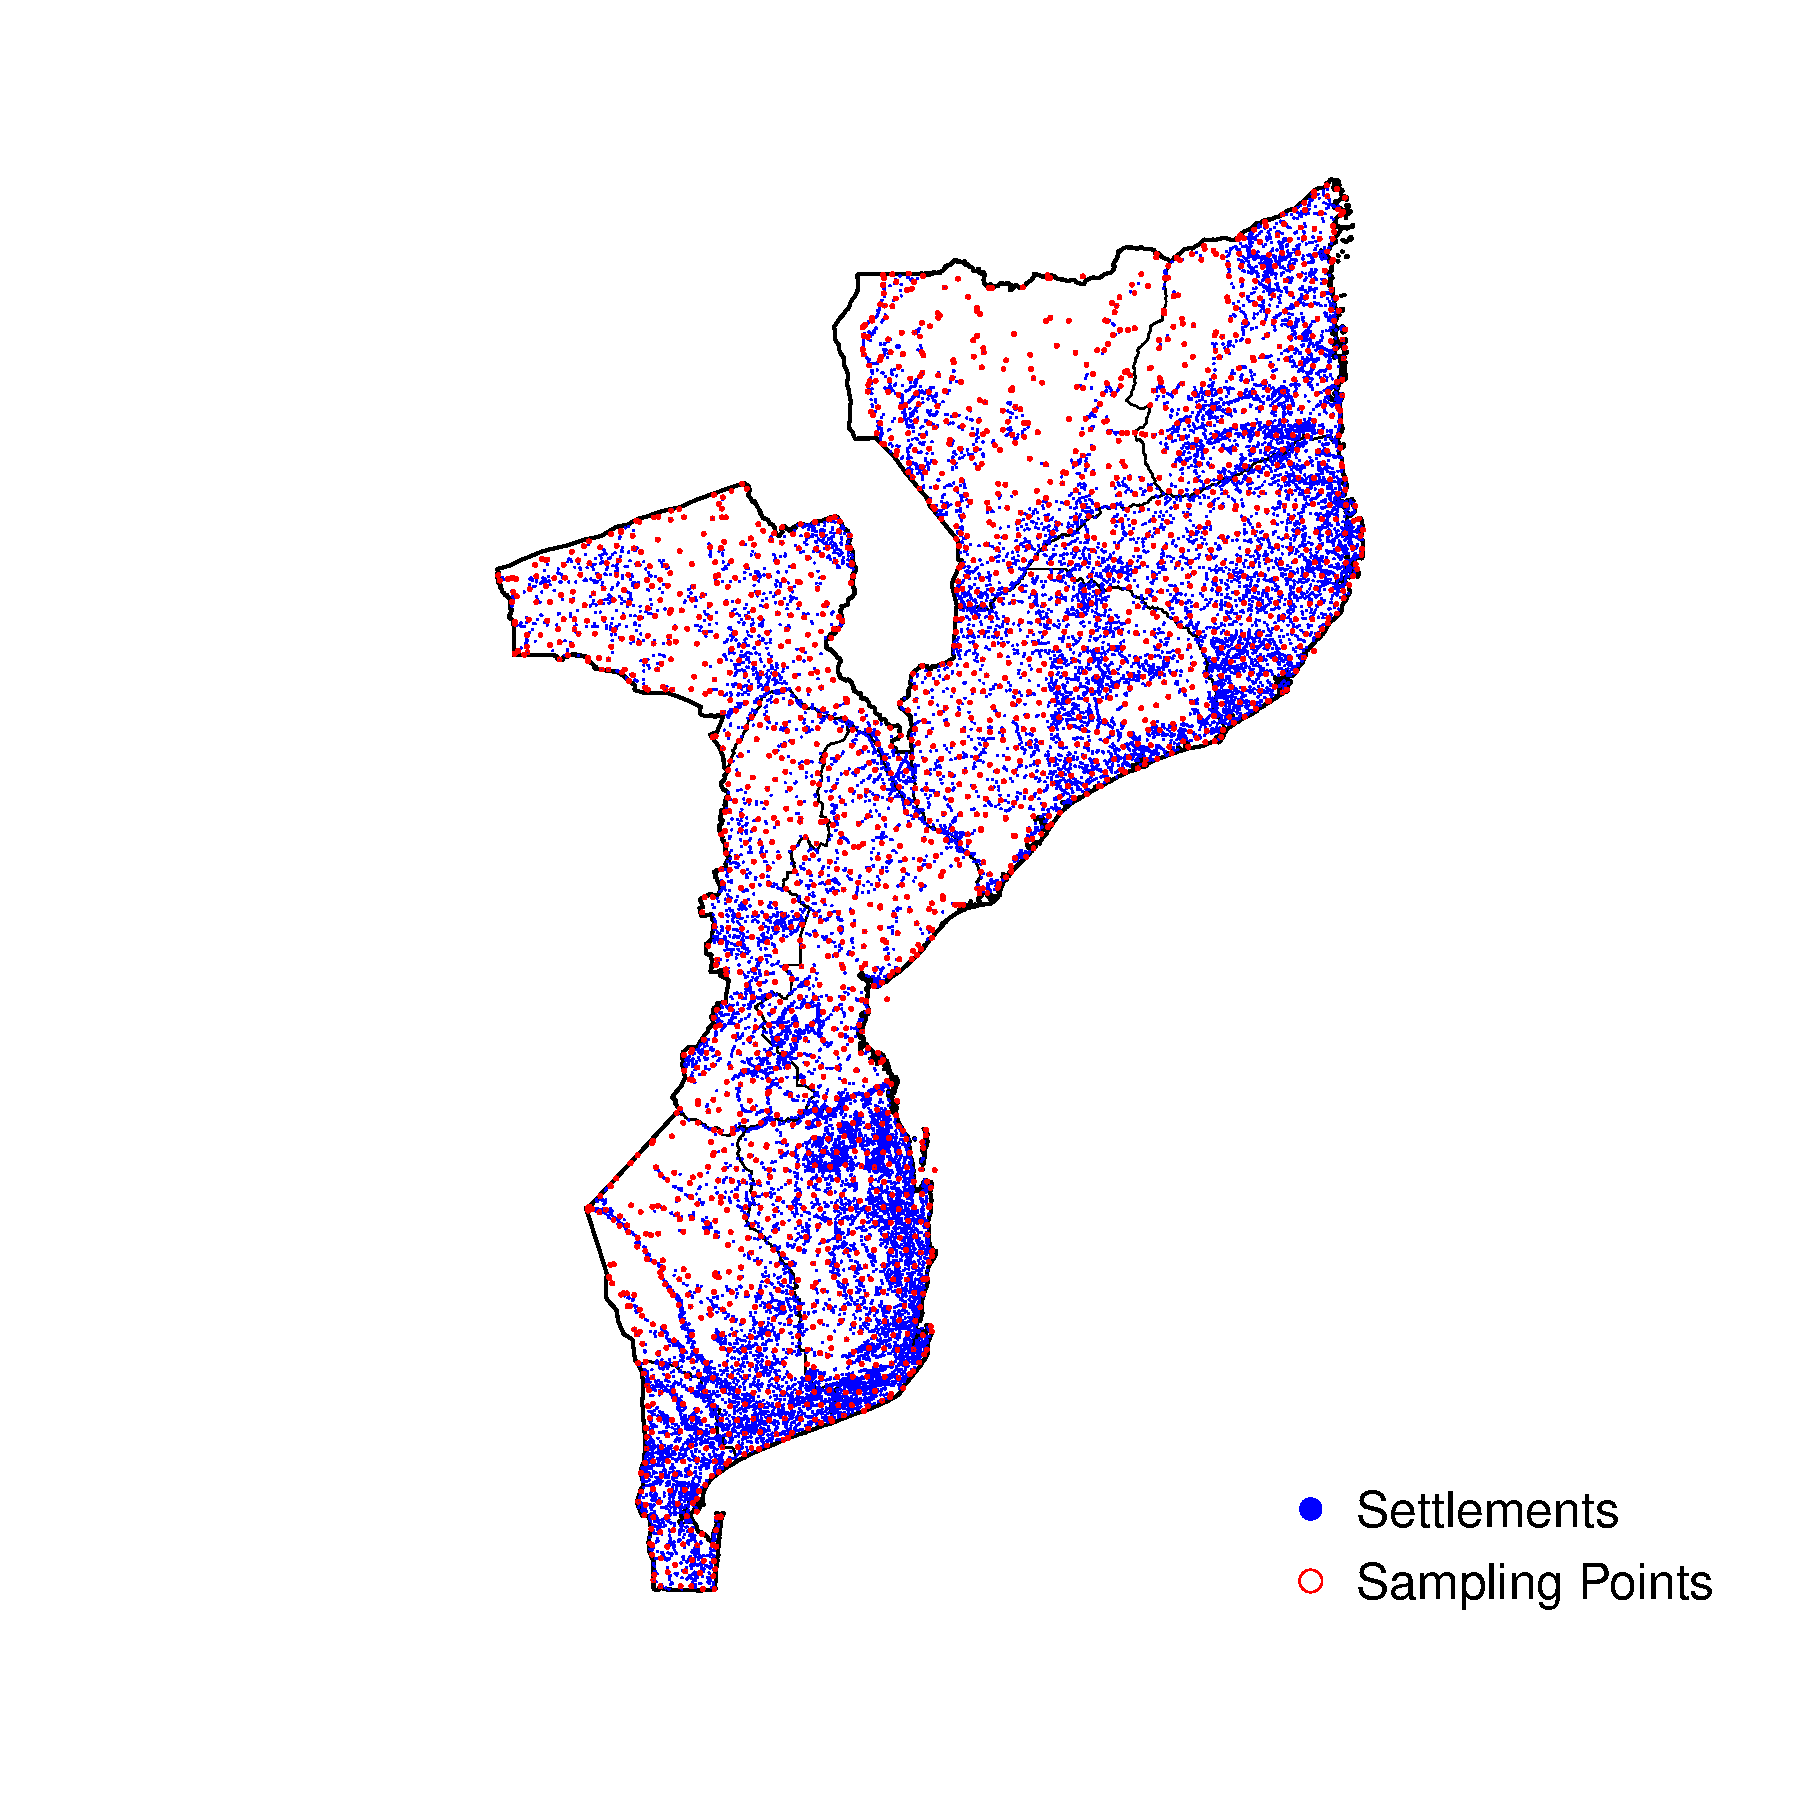
\includegraphics{mozambiqueNotes_files/figure-latex/stage1plot11-1} 

}

\caption{Stage 1 sampling map for d of 11 kms}\label{fig:stage1plot11}
\end{figure}

\begin{figure}[H]

{\centering 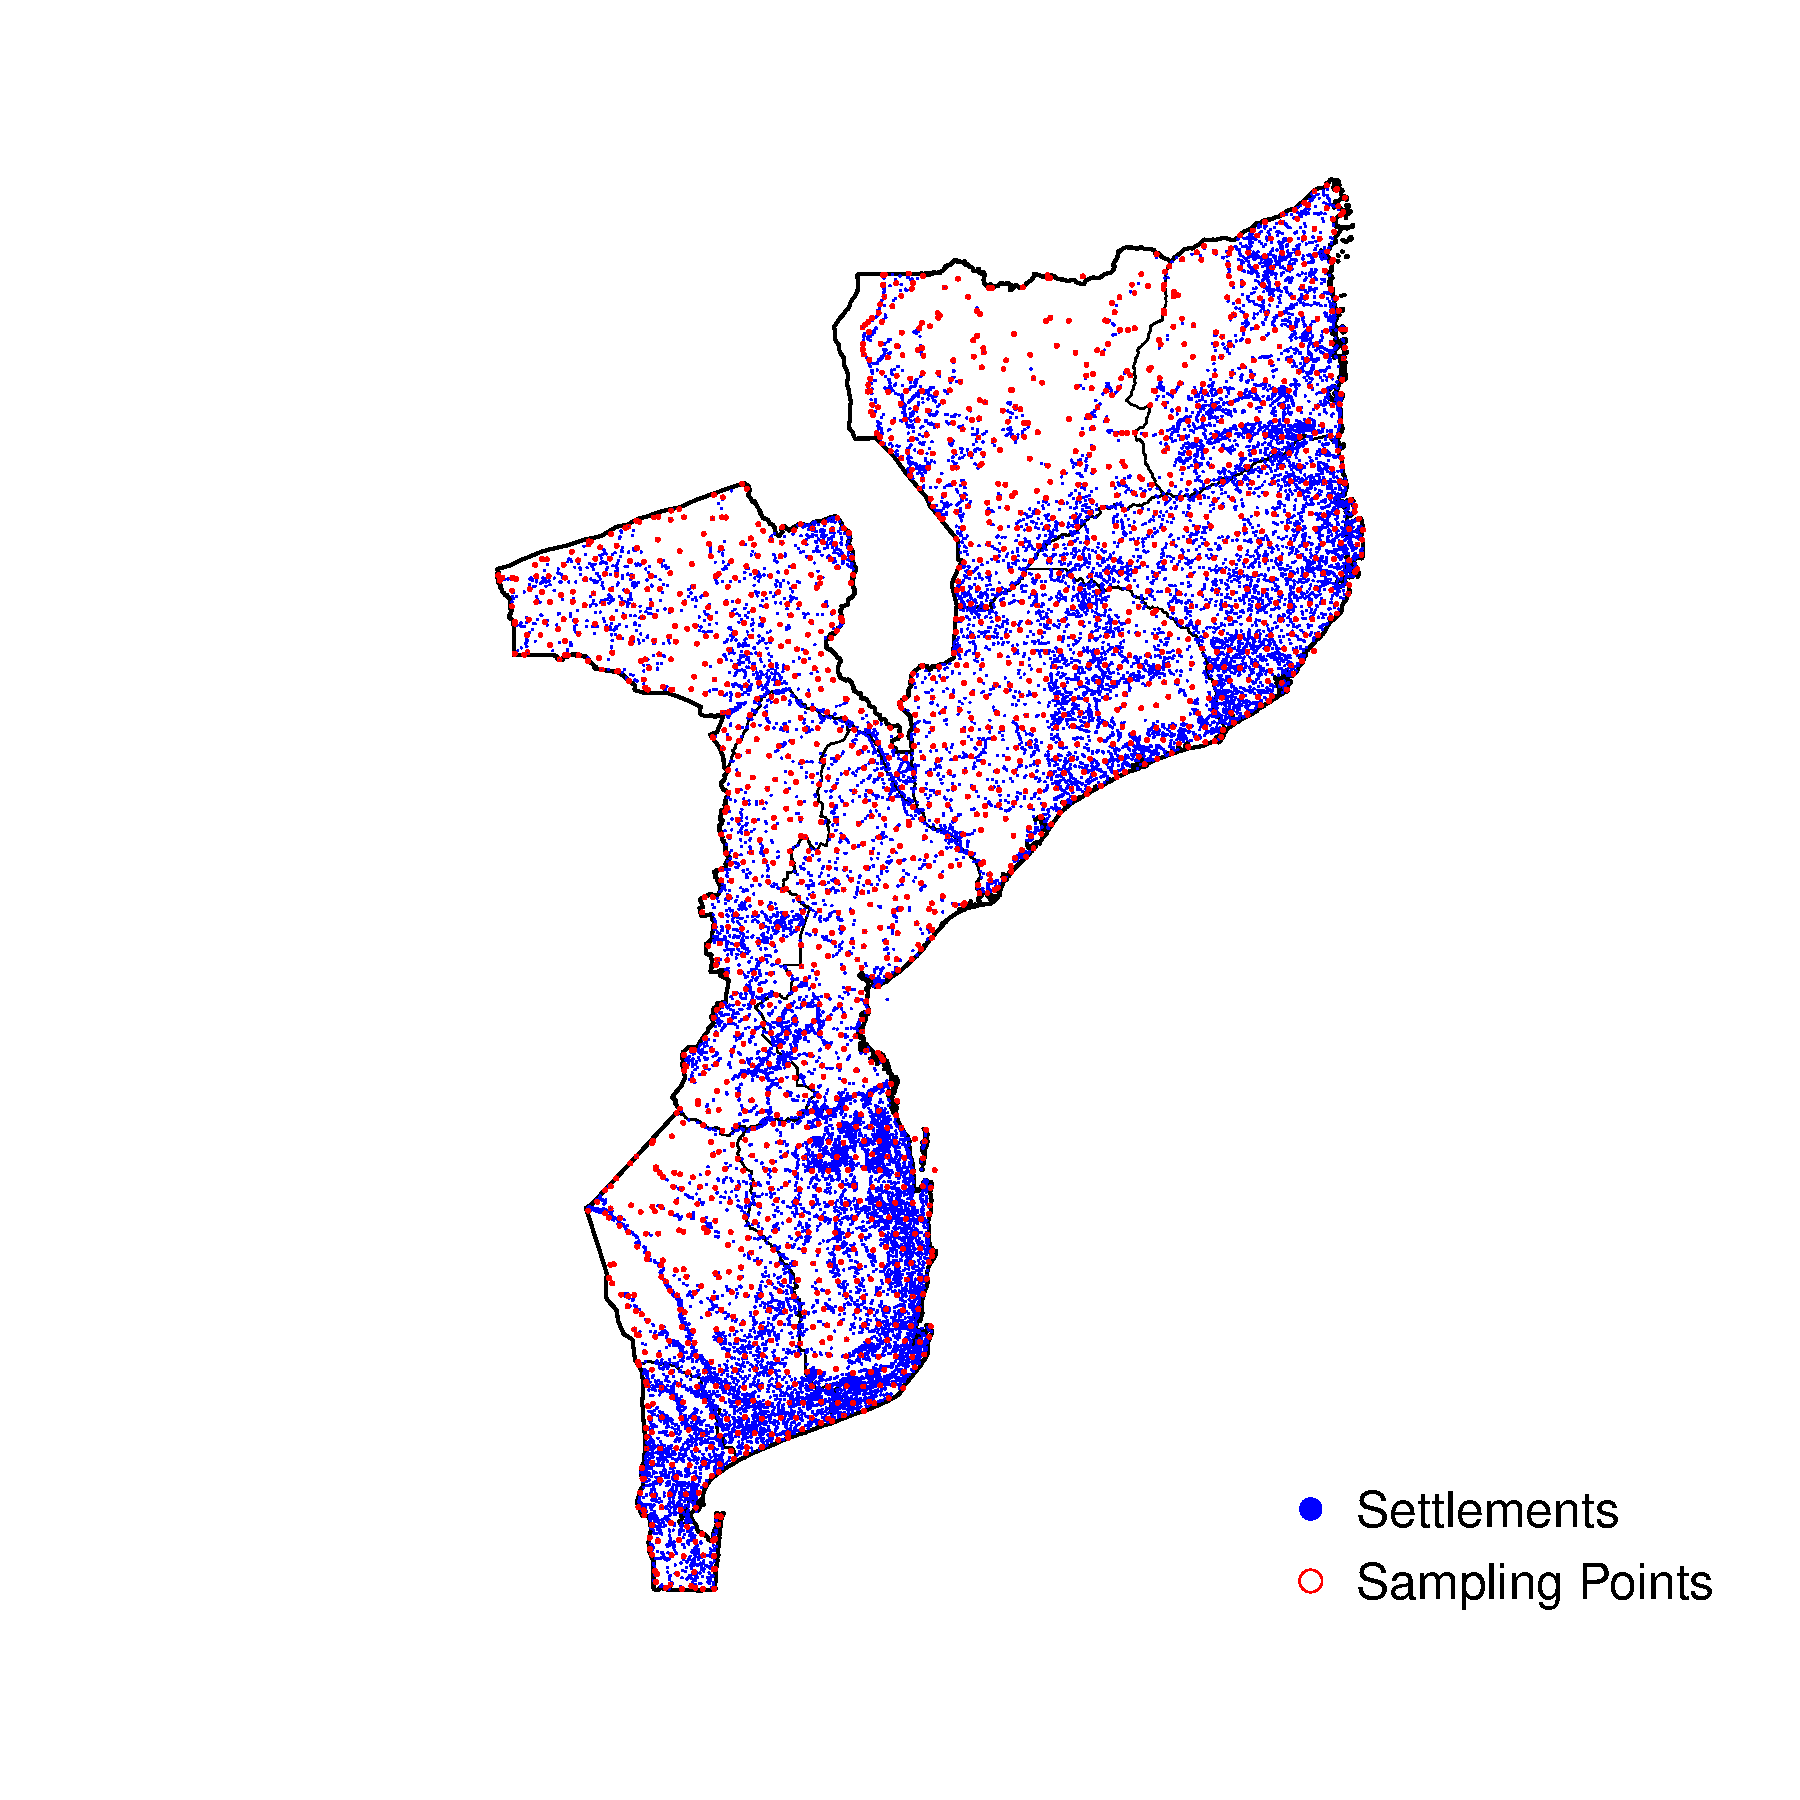
\includegraphics{mozambiqueNotes_files/figure-latex/stage1plot12-1} 

}

\caption{Stage 1 sampling map for d of 12 kms}\label{fig:stage1plot12}
\end{figure}

\begin{figure}[H]

{\centering 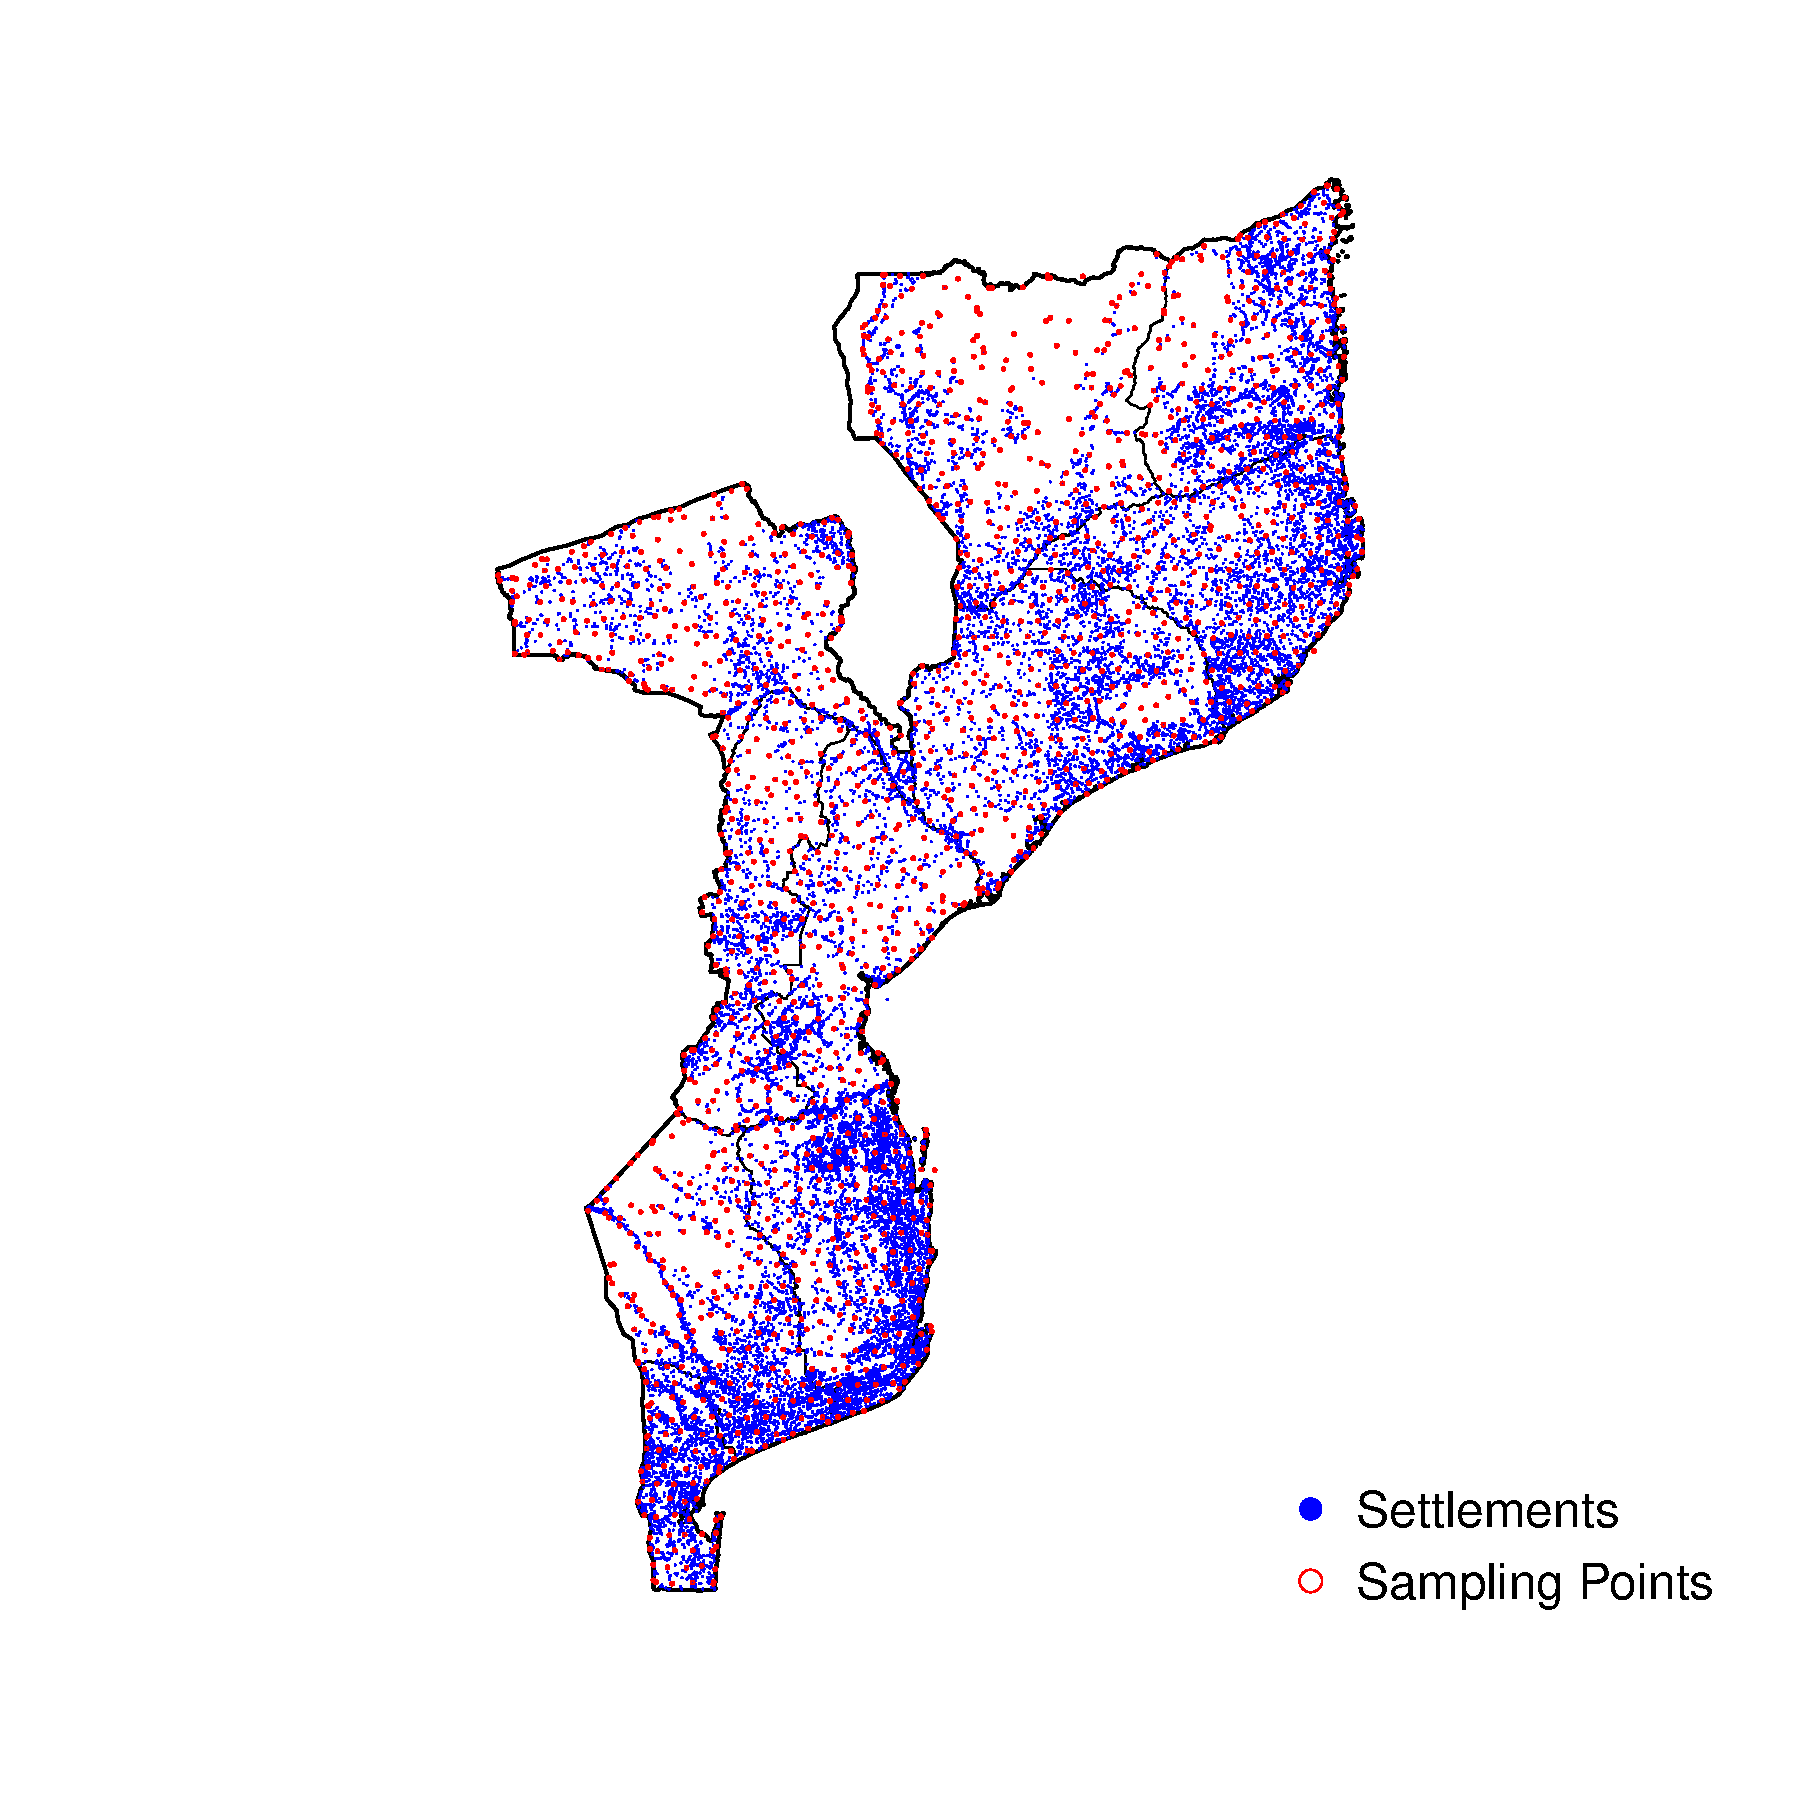
\includegraphics{mozambiqueNotes_files/figure-latex/stage1plot13-1} 

}

\caption{Stage 1 sampling map for d of 13 kms}\label{fig:stage1plot13}
\end{figure}

\begin{figure}[H]

{\centering 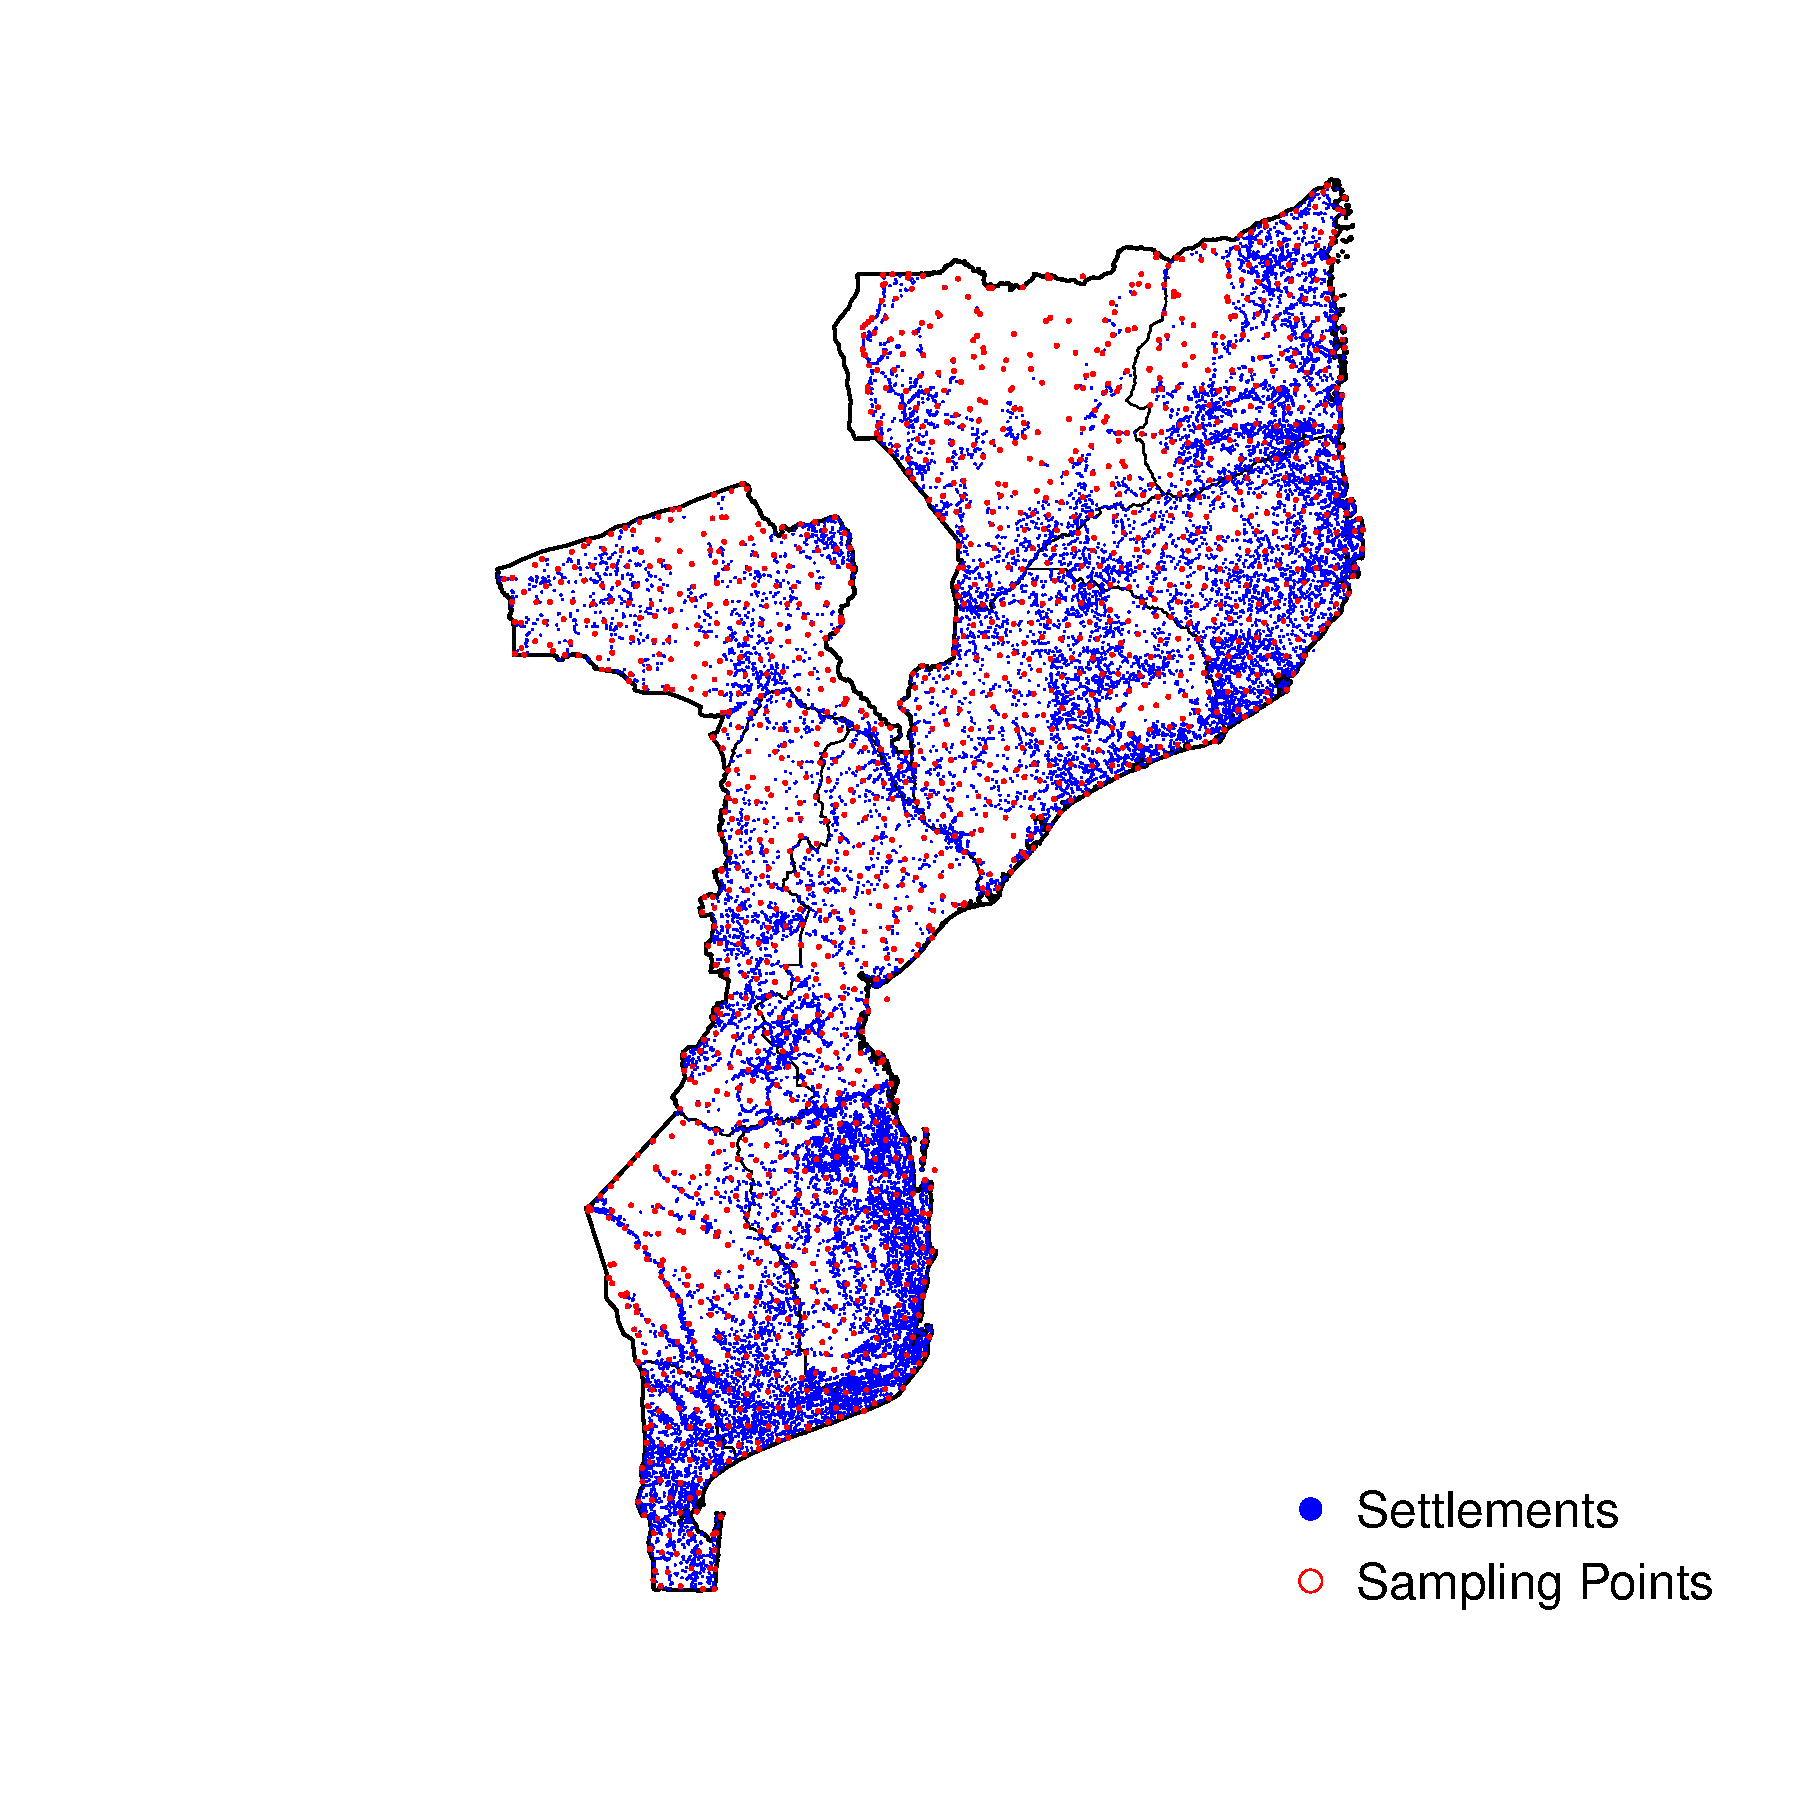
\includegraphics{mozambiqueNotes_files/figure-latex/stage1plot14-1} 

}

\caption{Stage 1 sampling map for d of 14 kms}\label{fig:stage1plot14}
\end{figure}

\begin{figure}[H]

{\centering 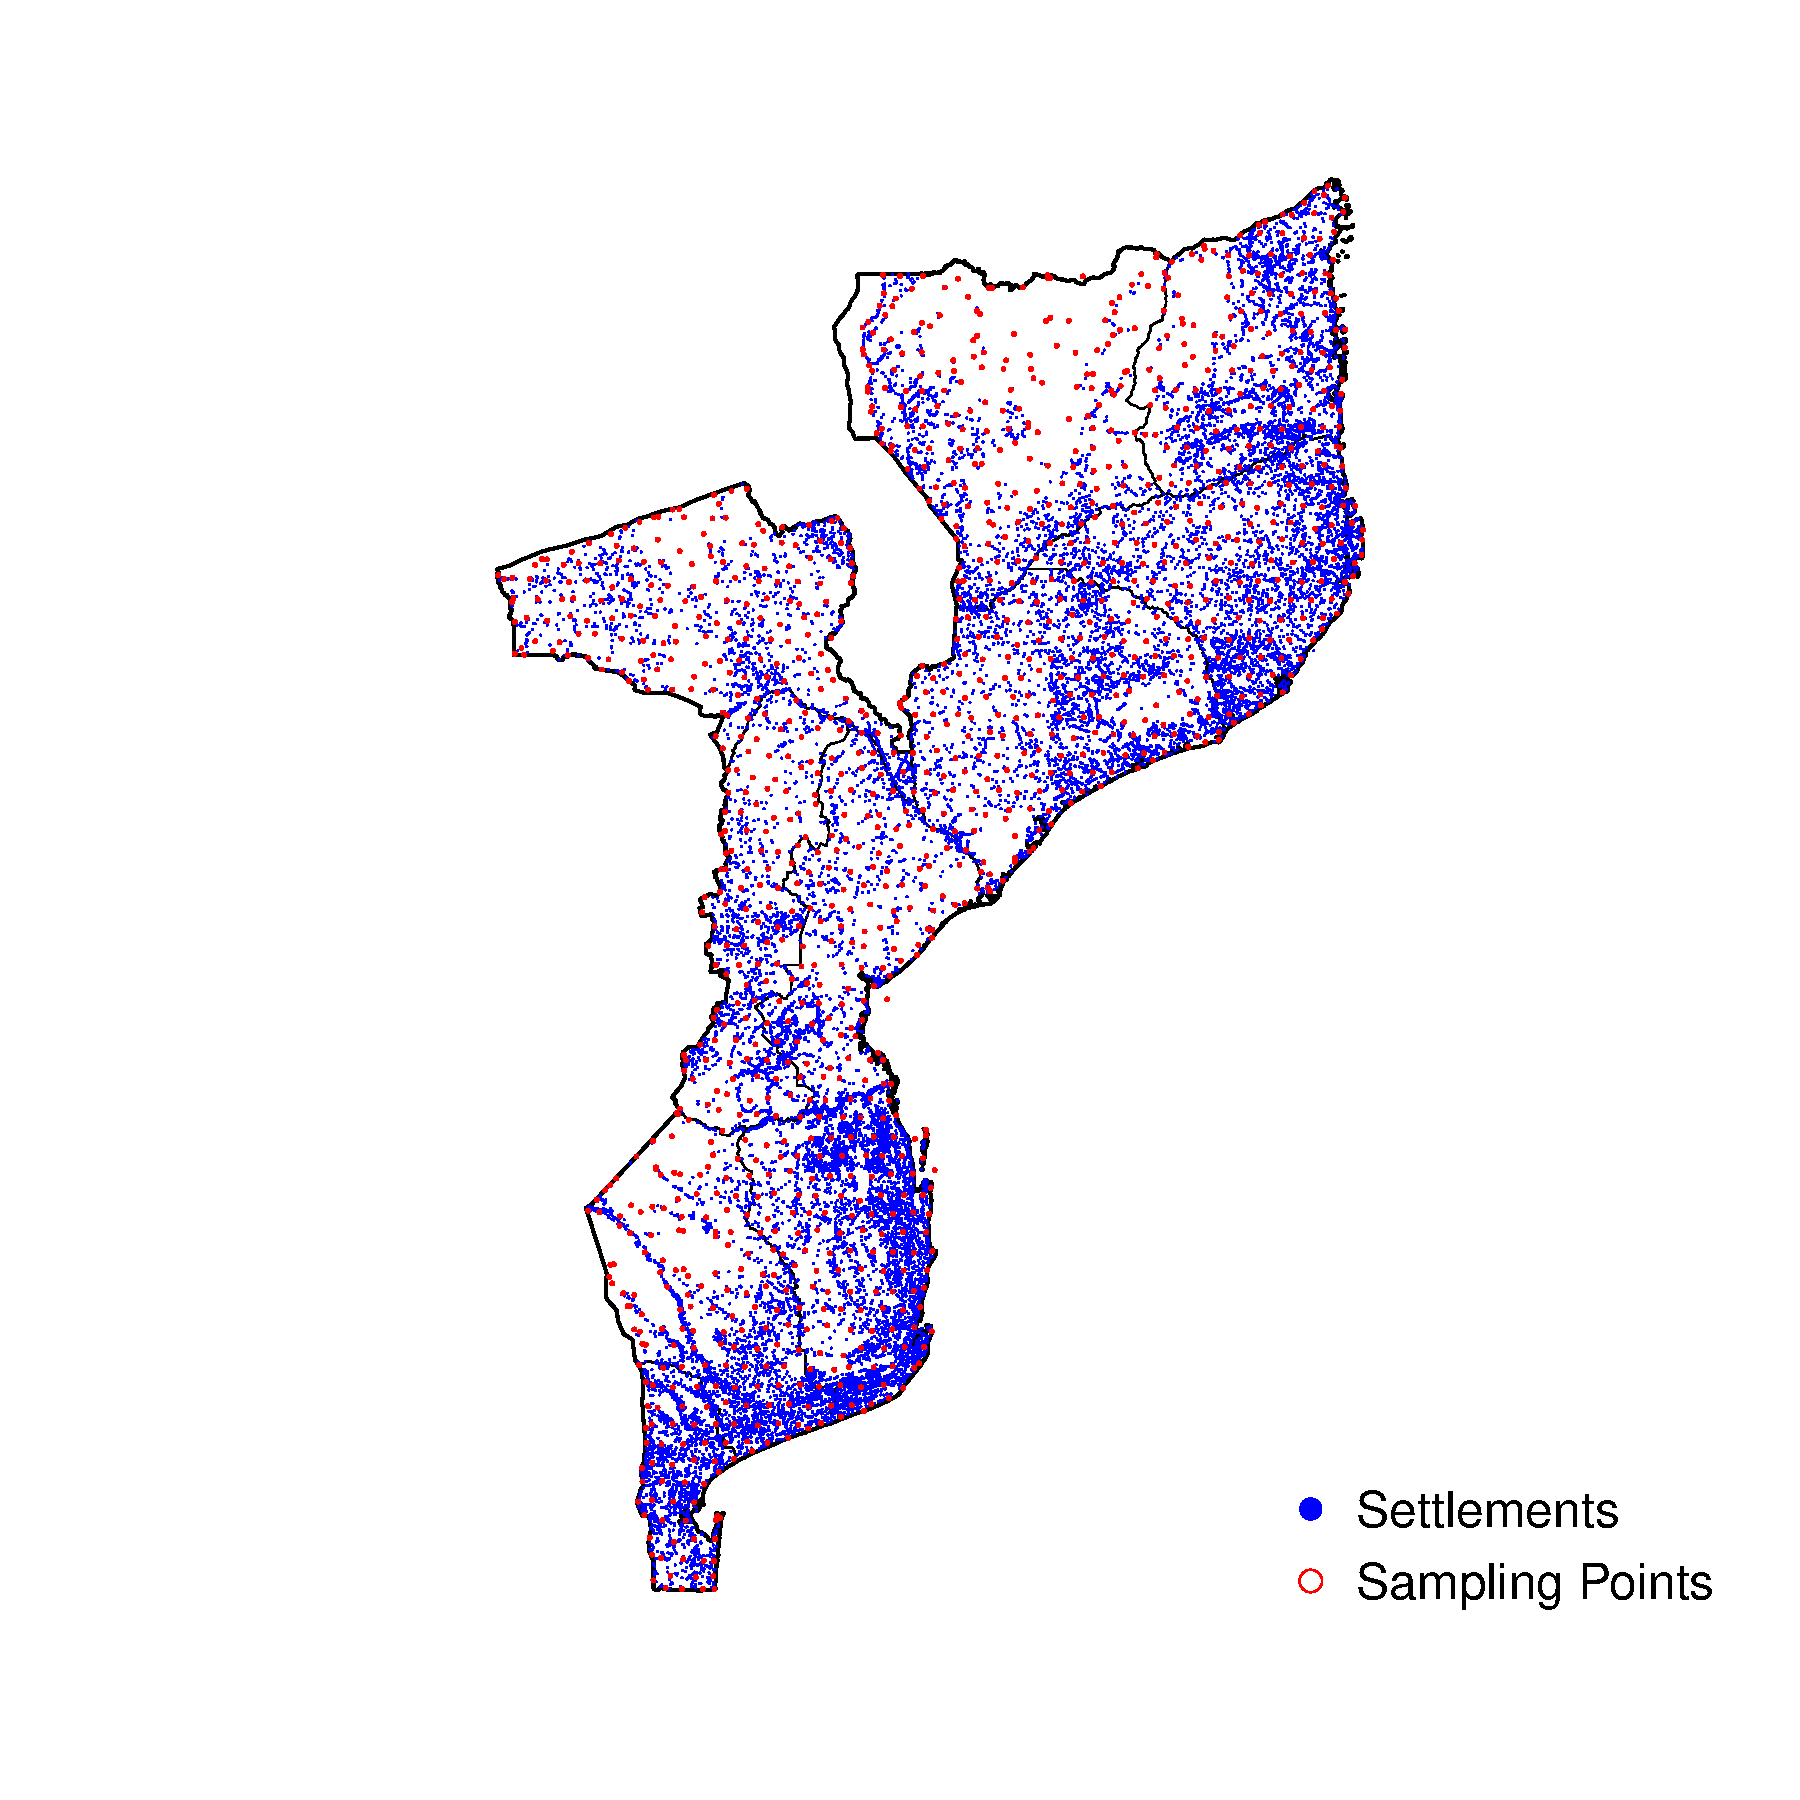
\includegraphics{mozambiqueNotes_files/figure-latex/stage1plot15-1} 

}

\caption{Stage 1 sampling map for d of 15 kms}\label{fig:stage1plot15}
\end{figure}

\hypertarget{determining-d-using-half-the-distance-between-markets-approach}{%
\subsection{Determining d using `half the distance between markets' approach}\label{determining-d-using-half-the-distance-between-markets-approach}}

Another possible approach to the determination of an appropriate value for \texttt{d} is the `half the distance between markets'. This method is described in the FANTA SQUEAC Technical Reference \citep{Myatt:2012tta}. In this approach, the value of \texttt{d} is approximated by the distance carers are willing to walk/travel to access services. A proxy for this would be the half the average distance of villages to the nearest market.

Using the locations of settlements, and the locations of major towns and cities in Mozambique, half the average distance to markets can be estimated as follows:

\begin{Shaded}
\begin{Highlighting}[]
\KeywordTok{library}\NormalTok{(mozambique)}
\KeywordTok{library}\NormalTok{(tripack)}
\KeywordTok{library}\NormalTok{(geosphere)}

\CommentTok{## location data for major towns and cities}
\NormalTok{townsCities <-}\StringTok{ }\KeywordTok{subset}\NormalTok{(ppl, place }\OperatorTok\StringTok{ }\KeywordTok{c}\NormalTok{(}\StringTok{"town"}\NormalTok{, }\StringTok{"city"}\NormalTok{))}

\CommentTok{## Get distance between towns and cities}
\NormalTok{distTownsCities <-}\StringTok{ }\KeywordTok{distm}\NormalTok{(}\DataTypeTok{x =}\NormalTok{ townsCities)}

\CommentTok{## Craete a triangular irregular network between towns and cities via }
\CommentTok{## Delaunay triangulation}
\NormalTok{triTownsCities <-}\StringTok{ }\KeywordTok{tri.mesh}\NormalTok{(}\DataTypeTok{x =}\NormalTok{ townsCities}\OperatorTok{@}\NormalTok{coords[ , }\DecValTok{1}\NormalTok{],}
                           \DataTypeTok{y =}\NormalTok{ townsCities}\OperatorTok{@}\NormalTok{coords[ , }\DecValTok{2}\NormalTok{])}

\CommentTok{## Get network of towns and cities}
\NormalTok{nbTownsCities <-}\StringTok{ }\KeywordTok{neighbours}\NormalTok{(triTownsCities)}

\CommentTok{## Get vector of distances in network of towns and cities}
\NormalTok{listDistances <-}\StringTok{ }\OtherTok{NULL}

\ControlFlowTok{for}\NormalTok{(i }\ControlFlowTok{in} \KeywordTok{seq_len}\NormalTok{(}\KeywordTok{length}\NormalTok{(nbTownsCities))) \{}
\NormalTok{  x <-}\StringTok{ }\OtherTok{NULL}
  \ControlFlowTok{for}\NormalTok{(j }\ControlFlowTok{in}\NormalTok{ nbTownsCities[[i]]) \{}
\NormalTok{    x <-}\StringTok{ }\KeywordTok{c}\NormalTok{(x, distTownsCities[i, j])}
\NormalTok{  \}}
\NormalTok{  listDistances <-}\StringTok{ }\KeywordTok{c}\NormalTok{(listDistances, x)}
\NormalTok{\}}

\CommentTok{## Convert distances to kms }
\NormalTok{listDistances <-}\StringTok{ }\NormalTok{listDistances }\OperatorTok{/}\StringTok{ }\DecValTok{1000}

\CommentTok{## Get half of median distance}
\KeywordTok{median}\NormalTok{(listDistances) }\OperatorTok{/}\StringTok{ }\DecValTok{2}
\end{Highlighting}
\end{Shaded}

\begin{verbatim}
## [1] 22.60953
\end{verbatim}

\begin{Shaded}
\begin{Highlighting}[]
\CommentTok{## Get half of the mean distance}
\KeywordTok{mean}\NormalTok{(listDistances) }\OperatorTok{/}\StringTok{ }\DecValTok{2}
\end{Highlighting}
\end{Shaded}

\begin{verbatim}
## [1] 34.52044
\end{verbatim}

In the calculations above, we use both median and mean. The half of the mean distance to markets is about \textbf{35 kms} while half the median distance to markets is about \textbf{23 kms}.

In this case, median might be the more robust estimator as there are some long distances along the borders of the triangular network that connects extremely distant points on the network.

If we use a \texttt{d} of 23 kms, we get the following stage 1 sampling frame:

\begin{table}[H]

\caption{\label{tab:halfdist3}Stage 1 sample characteristics for d values based on half distance between markets}
\centering
\begin{tabular}[t]{rrr}
\toprule
d & \makecell[c]{Number\\of\\sampling\\points} & \makecell[c]{Number\\of\\clusters/\\settlements\\selected}\\
\midrule
\rowcolor{gray!6}  23 & 584 & 589\\
35 & 252 & 252\\
\bottomrule
\end{tabular}
\end{table}

\begin{figure}[H]

{\centering 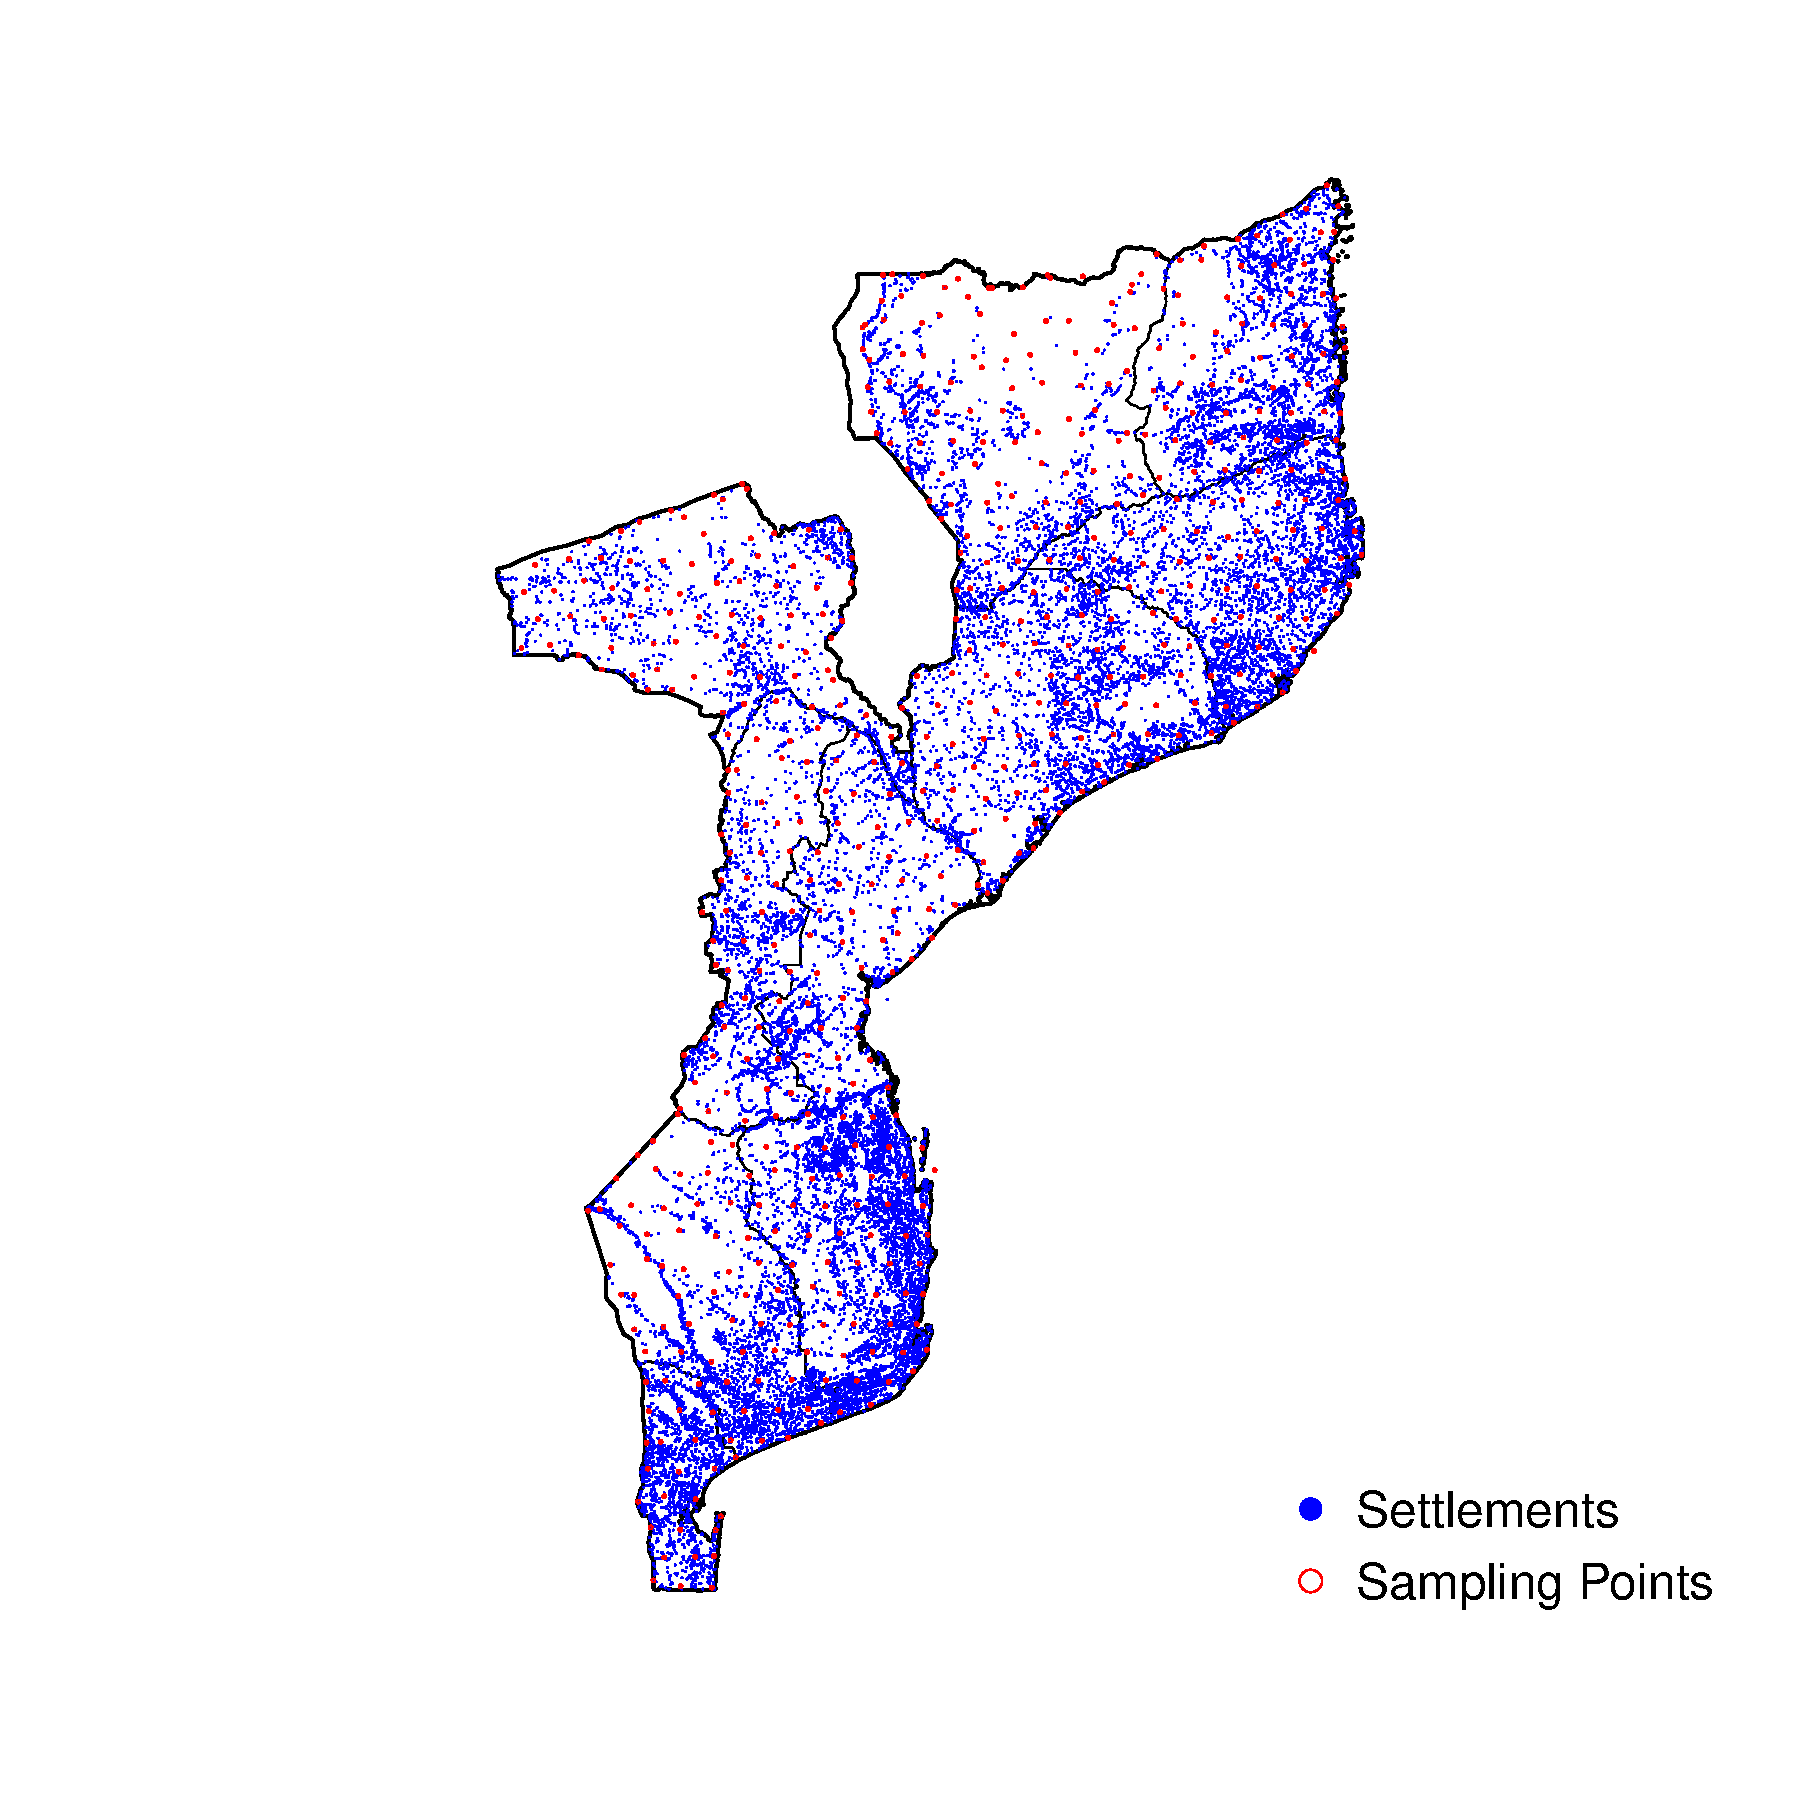
\includegraphics{mozambiqueNotes_files/figure-latex/stage1plot23-1} 

}

\caption{Stage 1 sampling map for d of 23 kms}\label{fig:stage1plot23}
\end{figure}

\begin{figure}[H]

{\centering 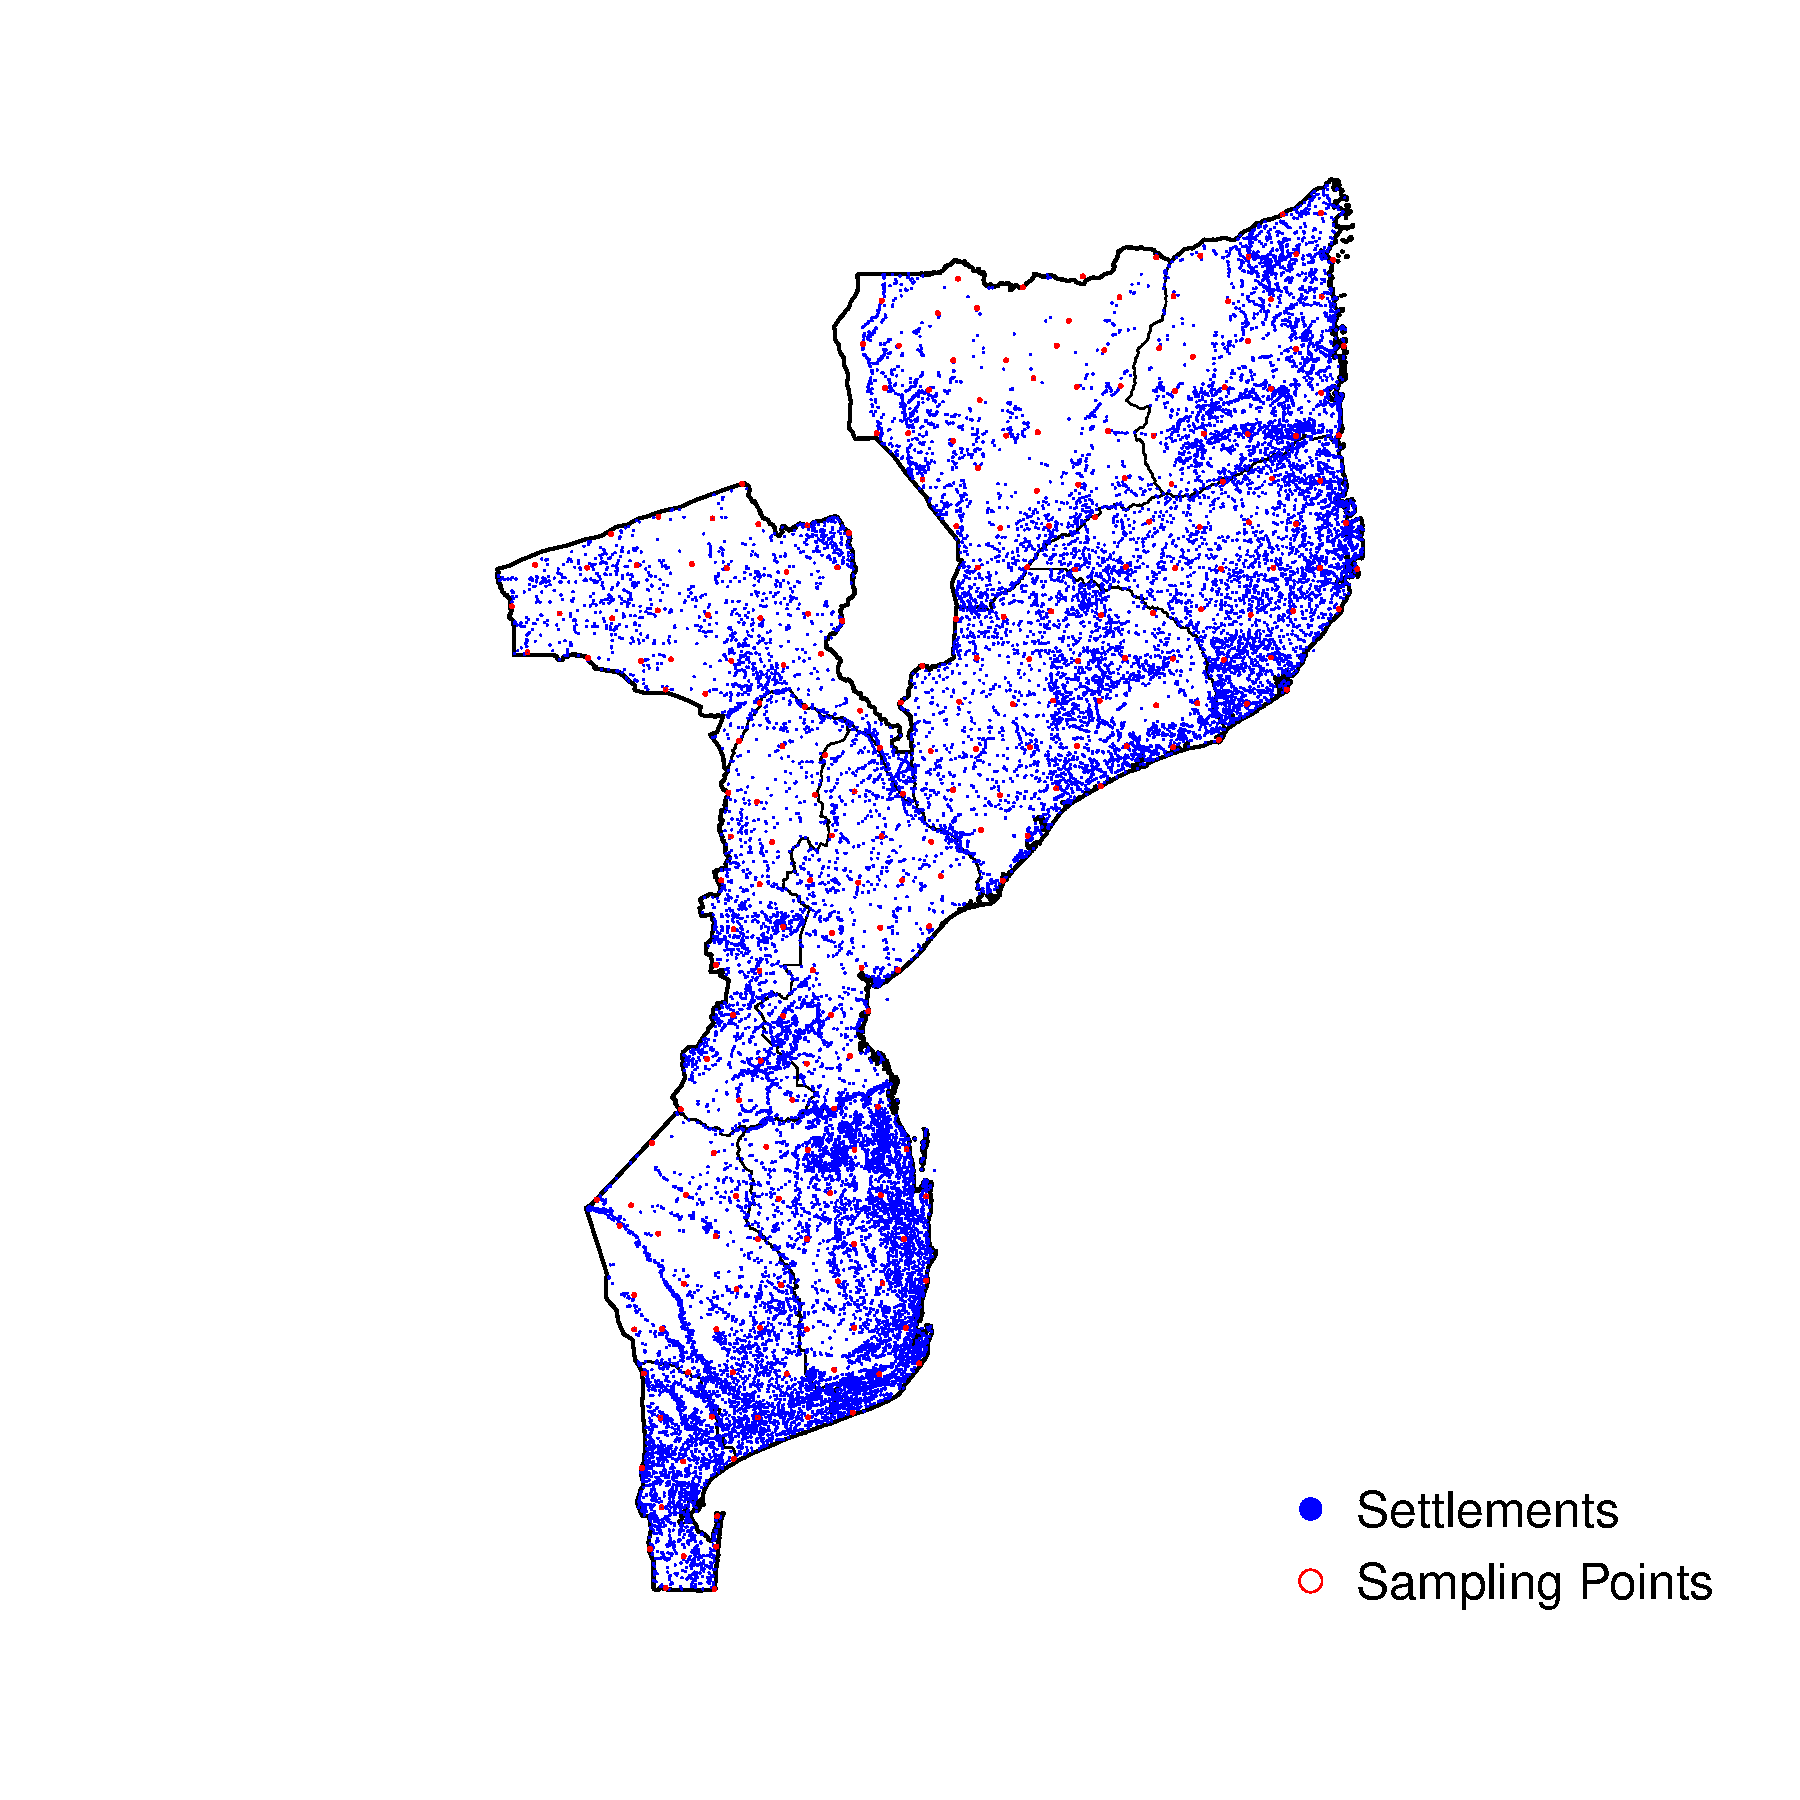
\includegraphics{mozambiqueNotes_files/figure-latex/stage1plot35-1} 

}

\caption{Stage 1 sampling map for d of 35 kms}\label{fig:stage1plot35}
\end{figure}

  \bibliography{bibliography.bib}

\end{document}
